\documentclass[11pt,a4paper]{ctexbook}
\setlength\topmargin{-48pt}
\setlength\headheight{0pt}
\setlength\headsep{25pt}
\setlength\marginparwidth{-20pt}
\setlength\textwidth{7.0in}
\setlength\textheight{9.5in}
\setlength\oddsidemargin{-30pt}
\setlength\evensidemargin{-30pt}


\frenchspacing						% better looking spacing

% Call packages we'll need
\usepackage{CJK,CJKnumb}
%usepackage[english]{babel}			% english
\usepackage{graphicx}				% images
\usepackage{amssymb,amsmath}		% math
\usepackage{multicol}				% three-column layout
\usepackage{url,ctex,tikz}					% clickable links
\usepackage{marvosym}				% symbols
\usepackage{wrapfig}				% wrapping text around figures
\usepackage[T1]{fontenc}			% font encoding
\usepackage{charter} 				% Charter font for main content
\usepackage{datetime}				% custom date
\usepackage{mdframed} 
\usepackage{lipsum}%ダミーの文章を入れる
\usepackage{capt-of}
\usepackage[margin=2cm]{geometry}
\usepackage{tcolorbox}
\usepackage{varwidth}
\usepackage{amsmath}
\usepackage{enumitem}
\usepackage{varwidth}
\usepackage{tikz}
\usepackage{pdfpages}
\usepackage{authblk}
\usepackage{mathrsfs}%\mathscr字体
\usepackage{esint}%环路积分
\usepackage[T1]{fontenc}
\usepackage{lmodern}%微元\dj
\usepackage{booktabs} %三线表
\usepackage{tabularx} %表格自动换行
%\usepackage{titlesec}
%\titleformat{\chapter}{\heiti\huge\bfseries\center}


% 使用 tocloft 宏包控制目录样式
%\usepackage{tocloft}

% 设置目录中条目和页码之间的点
%\renewcommand{\cftdotsep}{1}  % 设置点之间的间隔(1是较小的间隔值,默认9)
%\renewcommand{\cftchapleader}{\cftdotfill{\cftdotsep}}  % 章节标题使用点引导线
%\renewcommand{\cftsecleader}{\cftdotfill{\cftdotsep}}  % 小节标题使用点引导线

\ctexset{
    chapter = {
        format = \centering\Huge\bfseries\heiti,  % 字号和字体,例如:二号字,黑体
        name = {第, 章},           % 章节前后的文字,例:第1章
        number = \chinese{chapter},% 使用中文数字编号
        aftername = \quad          % 章节标题与数字之间的空隙
    }
}


\usetikzlibrary{calc}
\tcbuselibrary{breakable}
\tcbuselibrary{skins}
\tcbuselibrary{xparse}%xparse . sty定义的NewDocumentCommand
\usepackage{setspace}
\linespread{1.3}

\everymath{\displaystyle}


\usepackage{xpinyin}
\definecolor{frameinnercolor}{RGB}{0,112,131}%{249,179,72}


	\newdateformat{mydate}{\monthname[\THEMONTH] \THEYEAR}
\usepackage[pdfpagemode=FullScreen,
			colorlinks=false]{hyperref}	% links and pdf behaviour


%————版面设置————%
\usepackage{fancyhdr}
\renewcommand{\headrulewidth}{0.4pt}
\renewcommand{\headwidth}{\textwidth}
\renewcommand{\footrulewidth}{0pt}

\usepackage{physics}

\usepackage{gbt7714}
\newtheorem{definition}{\hspace{2em}定义}[chapter]
\newtheorem{theorem}{\hspace{2em}定理}[chapter]
\newtheorem{law}{\hspace{2em}定律}[chapter]
\newtheorem{equa}{\hspace{2em}公式}[chapter]
\newtheorem{lemma}{\hspace{2em}引理}[chapter]
\newtheorem{proof}{证明}[chapter]
\newtheorem{proposition}{\hspace{2em}命题}[chapter]
\newtheorem{corollary}{\hspace{2em}推论}[chapter]
\newtheorem{remark}{\hspace{2em}注}[chapter]

\newcommand{\pp}{\partial}%偏导数
\newcommand{\me}{\mathrm e}%自然底数
\newcommand{\mi}{\mathrm i}%虚数单位
\newcommand{\mj}{\mathrm j}%虚数单位
\newcommand{\mk}{\mathrm k}%虚数单位
\newcommand{\dps}{\displaystyle}%行间公式
\newcommand{\degree}{^\circ}%角度
\renewcommand{\bar}{\overline}%平均值
\renewcommand{\vec}{\boldsymbol}%粗体向量
%\renewcommand{\vec}{\overrightarrow}%向量箭头

\newcounter{problem}
\setcounter{problem}{0}
\newcommand{\problem}[1]{%
        \refstepcounter{problem}%
        {\bfseries{\thechapter.\theproblem\quad } #1}%
    \vspace{3pt}%
}

\newtheorem{solution}{参考解答}[chapter]

\title{\huge \heiti{高显经典力学习题解答}}
\author{ \ttfamily \texttt \Large 数据风暴中的避风港\\}
\date{\large \today}

\renewcommand{\today}{二〇二五年\CJKnumber\month 月\CJKnumber\day 日}

\begin{document}
\maketitle

\pagestyle{fancy}
\fancyhf{}
\fancyhead{}
~\vfill
\noindent \textit{数据风暴中的避风港 }\textsc{ 社区成员共同编写, 本习题解答及其\LaTeX 代码符合 MIT 许可.}\\

\noindent \textsc{链接:\url{https://github.com/Phiyu/GaoXian}}.\\

\noindent \textsc{编写成员均为物理专业或非物理专业的物理爱好者, 编写过程中难免有许多纰漏, 欢迎指出, 也欢迎加入}
\textit{ 数据风暴中的避风港 } 
\textsc{大家庭(QQ群:832100706) .}\\

\noindent \textit{\number\year 年 \number\month 月} % Printing/edition date

\tableofcontents

\newpage
\pagestyle{fancy}
\fancyhf{} 
\fancyhead[LE]{\kaishu \leftmark}
\fancyhead[RE]{\kaishu 习题解答}
\fancyhead[RO]{\kaishu \leftmark}
\fancyhead[LO]{\kaishu 习题解答}
\fancyfoot[LE]{\kaishu 高显经典力学习题解答}
\fancyfoot[RE]{\kaishu 数据风暴中的避风港}
\fancyfoot[LO]{\kaishu 数据风暴中的避风港}
\fancyfoot[RO]{\kaishu 高显经典力学习题解答}
\cfoot{\thepage}

\pagenumbering{arabic}
\setcounter{page}{1}

\setcounter{problem}{0}
\newpage
\chapter{变分法}
\problem{给定\(f(t)\)的泛函\[S[f]=-\int \dd t\,\me^{-V(f(t))} \sqrt{1-(f'(t))^2}\]其中\(V\)是\(f\)的任意函数. 求\(S[f]\)取极值时, \(f(x)\)的欧拉-拉格朗日方程.}
\begin{solution}
    记 $L = \me^{-V(f(t))} \sqrt{1-(f'(t))^2}$, 则
    \[
        \frac{\pp L}{\pp f} = V \frac{\dd V}{\dd f} \me^{-V(f(t))} \sqrt{1-(f'(t))^2}, \qquad 
        \frac{\pp L}{\pp f'} = \me^{-V(f(t))} \frac{f'(t)}{\sqrt{1-(f'(t))^2}}
    \]
    \[
    \begin{aligned}
        \delta S &= \int \dd t\,\left(V \frac{\dd V}{\dd f} \me^{-V(f(t))} \sqrt{1-(f'(t))^2} \delta f + \me^{-V(f(t))} \frac{f'(t)}{\sqrt{1-(f'(t))^2}} \delta f'\right)\\
        &\simeq \int \dd t\,\left(V \frac{\dd V}{\dd f} \me^{-V(f(t))} \sqrt{1-(f'(t))^2} - \frac{\dd}{\dd t}\left(\me^{-V(f(t))} \frac{f'(t)}{\sqrt{1-(f'(t))^2}}\right)\right) \delta f
    \end{aligned}
    \]
    因此, Euler-Lagrange 方程为
    \[
        - \frac{\delta S}{\delta f} = - V \frac{\dd V}{\dd f} f' \me^{-V(f(t))} \frac{f'}{\sqrt{1-f'^2}} + \me^{-V(f(t))} \frac{f'' + (1-f')f'^2}{(1 - f'^2)^{3/2}} - V \frac{\dd V}{\dd f} \me^{- V(f(t))} \sqrt{1-f'^2} = 0
    \]
\end{solution}

\problem{给定\(f(t)\)的泛函\(S[f] = \int \dd t\,L\), 其中\(L = (f'(t))^2 + f(t) f'(t)+ \frac{1}{2} f(t) f''(t)\).\\[-0.8em]
    \begin{enumerate}[label=(\arabic*)]
        \item 求一阶泛函导数\(\frac{\delta S}{\delta f}\);
        \item 将\(L\)改写成\(L = \tilde{L} + \frac{\dd F}{\dd t}\)的形式, 要求\(\tilde{L}\)中不包含\(f''(t)\), 求\(\tilde{L}\)和\(F\);
        \item 求泛函\(\tilde{S}[f] = \int \dd t\,\tilde{L}\)的一阶泛函导数\(\frac{\delta \tilde{S}}{\delta f}\), 并比较其和\(\frac{\delta S}{\delta f}\)的异同.
    \end{enumerate}}
\begin{solution}
    \begin{enumerate}[label=(\arabic*)]
        \item     \[
            \begin{aligned}
                \delta S = \int \dd t\,\delta L &= \int \dd t \left(\left(f' + \frac{1}{2}f''\right)\delta f + \left(2f' + f\right)\delta f' + \frac{1}{2}f \delta f''\right)\\
                &\simeq \int \dd t \left(f' + \frac{1}{2}f'' - \frac{\dd}{\dd t}\left(2f'+f\right)+\frac{\dd^2}{\dd t^2}\left(\frac{1}{2}f\right)\right) \delta f \\
                \frac{\delta S}{\delta f} &= - f''
            \end{aligned}
            \]
        \item 假设\(F = \frac{1}{2}f f'\), 则\(\frac{\dd F}{\dd t} = \frac{1}{2}f'^2 + \frac{1}{2} f f''\), \(\tilde{L} = f f' + \frac{1}{2}f'^2\)满足题意.
        \item \[
        \begin{aligned}
            \delta \tilde{S}[f] &= \int \dd t \delta \tilde{L} = \int \dd t \left(f' \delta f + (f + f') \delta f'\right) \\
            &\simeq \int \dd t \left(f' - \frac{\dd}{\dd t} (f + f')\right)\delta f \\
            \frac{\delta \tilde{S}}{\delta f} &= - f''
        \end{aligned}
        \]
        注意到\(\frac{\delta \tilde{S}}{\delta f} = \frac{\delta S}{\delta f}\). 
    \end{enumerate}
\end{solution}

\problem{给定两个函数\(n(t)\)和\(a(t)\)的泛函\(S[n,a] = \int_{t_1}^{t_2} \dd t\,na^3\left(A(n) + 3 B(n) \frac{a'^2}{n^2 a^2}\right)\), 其中\(A, B\)是\(n(t)\)的任意函数. 求泛函\(S[n,a]\)取极值时, \(n(t)\)和\(a(t)\)的欧拉-拉格朗日方程.}
\begin{solution}
    \[
        \begin{aligned}
            \delta S & = \int \dd t \left(a^3\left(A(n) + 3B(n) \frac{a'^2}{n^2 a^2}\right) + n a^3 \left(\frac{\dd A}{\dd n} + 3\frac{\dd B}{\dd n}\frac{a'^2}{n^2 a^2} - \frac{3}{2}B(n)\frac{a'^2}{n^3 a^2}\right)\right) \delta n\\
            -\frac{\delta S}{\delta n} & = -a^3 A - 3B \frac{a a'^2}{n^2} - n a^3 \frac{\dd A}{\dd n} - 3n \frac{\dd B}{\dd n} \frac{a a'^2}{n^2} + \frac{3}{2}nB\frac{a a'^2}{n^3} = 0
        \end{aligned}
    \]
    \[
        \begin{aligned}
            \delta S & = \int \dd t \left(6 B \frac{a a'}{n} \delta a' + \left(3 n A a^2 + 3 B \frac{a'^2}{n}\right)\delta a\right) \\
            & \simeq \int \dd t \left(- \frac{\dd}{\dd t}\left(6 B \frac{a a'}{n}\right) + 3 n A a^2 + 3 B \frac{a'^2}{n}\right) \delta a \\
            - \frac{\delta S}{\delta a} & = \frac{\dd}{\dd t}\left(6 B \frac{a a'}{n}\right) - 3 n A a^2 - 3 B \frac{a'^2}{n} = 0
        \end{aligned}
    \]
\end{solution}

\problem{给定二元函数\(f(t,x)\)的泛函\(S[f]=\iint \dd t \dd x \frac12 \left[
    \left(\frac{\pp f(t,x)}{\pp t}\right)^2 - \left(\frac{\pp f(t,x)}{\pp x}\right)^2 -m^2f^2(t,x)
\right]\), 其中\(m\)是常数. 求泛函\(S[f]\)取极值时\(f(t,x)\)的欧拉-拉格朗日方程. }
\begin{solution}
    泛函\(S[f]\)的Lagrange函数为\(L(t,x,f,f_t,f_x) = \frac12(f_t^2-f_x^2-m^2f^2)\), 则
    \[
    \begin{aligned}
        \delta S & = \iint \dd t \dd x \delta L \\
                 & \simeq \iint \dd t \dd x \left[
                    \frac{\pp L}{\pp f} - \frac{\pp}{\pp t}\left( \frac{\pp L}{\pp f_t} \right) - \frac{\pp}{\pp x}\left( \frac{\pp L}{\pp f_x} \right)
                    \right] \\
                 & = \iint \dd t \dd x  
                 (-m^2f - f_{tt} + f_{xx})
                 \delta f
    \end{aligned}
    \]
    取极值有\(-\frac{\delta S}{\delta f}=0\), 即\(f_{tt} - f_{xx} + -m^2f = 0\)
\end{solution}

\problem{考虑一条不可拉伸、质量均匀的柔软细绳, 长为\(l\), 质量为\(m\). 细绳两端点悬挂于相同高度, 水平距离为\(a\)(\(a<l\)). 
    \begin{enumerate}[label=(\arabic*)]
        \item 选择合适的坐标, 求细绳总的重力势能\(V\)作为细绳形状的泛函; 
        \item 求细绳重力势能取极值时, 细绳形状所满足的欧拉-拉格朗日方程. 
    \end{enumerate}}
\begin{solution}
    \begin{enumerate}[label=(\arabic*)]
        \item 取细绳所在平面建立笛卡尔系, 设悬点为\( \vec{x_1}=(0,0) \), \( \vec{x_2}=(a,0) \), 
        竖直向下为\(y\)轴正方向, 设细绳形状为\( y=y(x) \) ( \( 0 \leq x \leq a \) ), 可知细绳线密度为\( \lambda = \frac{m}{l} \), 则
        \[
        \begin{aligned}
            V[y] &= \int -(\lambda \dd L) gy \\
                 &= -\frac{mg}{l} \int_0^a y\sqrt{1+y'^2} \dd x
        \end{aligned}
        \]
        \item 泛函\(V[y]\)的Lagrange函数为\( L(x,y,y')=-\frac{mg}{l}y\sqrt{1+y'^2} \), 重力势能取极值有
        \[
        \begin{aligned}
            -\frac{\delta V}{\delta y} &= \frac{\dd}{\dd x} \left( \frac{\pp L}{\pp y'} \right) - \frac{\pp L}{\pp y} \\
                                 &= -\frac{mg}{l} \left[  
                                 \frac{\dd}{\dd x} \left( \frac{yy'}{\sqrt{1+y'^2}} \right) - \sqrt{1+y'^2} 
                                 \right] \\
                                 &= -\frac{mg}{l} \left( 
                                 \frac{y'^2}{\sqrt{1+y'^2}} + \frac{yy''}{\sqrt{1+y'^2}} - \frac{yy'^2y''}{ (1+y'^2)^{3/2} } - \sqrt{1+y'^2} 
                                 \right) = 0
        \end{aligned}
        \]
        将最后一式化简得到:\( yy'' - y'^2 - 1 = 0 \) , 此即著名的悬链线满足的微分方程. 
    \end{enumerate}
\end{solution}

\problem{考虑3维欧氏空间中的任意2维曲面, 取直角坐标, 曲面方程为\( z=z(x,y) \). 曲面上任意两
    固定点, 由曲面上的任一曲线连接. 曲线方程为\( x=x(\lambda) \), \( y=y(\lambda) \), 这里的
    \( \lambda \)是曲线的参数. 
    \begin{enumerate}[label=(\arabic*)]
        \item 求曲线的长度\(S\)作为\( x(\lambda) \)和\( y(\lambda) \)的泛函\( S[x,y] \); 
        \item 求曲线长度\(S\)取极值时, \( x(\lambda) \)和\( y(\lambda) \)的欧拉-拉格朗日方程; 
        \item 当曲面为以下情况时, 求解\( x(\lambda) \)和\( y(\lambda) \):
        \begin{enumerate}[label=(\arabic{enumi}.\arabic*)]
            \item 平面\( z = ax + by + c \) ( \(a\), \(b\), \(c\)为常数 ); 
            \item 球面\( z = \sqrt{R^2 - x^2 - y^2} \) ( \(R\)为常数 ); 
            \item 锥面\( z = H \left( 1-\frac{1}{R}\sqrt{x^2+y^2} \right) \) ( \(H\), \(R\)为常数 ). 
        \end{enumerate}
    \end{enumerate}}
\begin{solution}
    \begin{enumerate}[label=(\arabic*)]
        \item \(S[x,y] = \int \dd \lambda \sqrt{x'^2 + y'^2} = \int \dd \lambda L\left(x',y'\right)\)
        \item 先对\(x(\lambda)\)做变分, \[
        \begin{aligned}
            \delta S = \int \dd \lambda \left(\frac{\pp L}{\pp x'} \delta x'\right) &= \int \dd \lambda \left(\frac{x'}{\sqrt{x'^2+y'^2}}\right) \delta x' \\
            &\simeq \int \dd \lambda \left(- \frac{\dd}{\dd \lambda} \frac{x'}{\sqrt{x'^2+y'^2}}\right) \delta x
        \end{aligned}
        \]
        因此, \(x(\lambda)\)的Euler-Lagrange方程为
        \[
            -\frac{\delta S}{\delta x} = \frac{\dd}{\dd \lambda} \left( \frac{x'}{\sqrt{x'^2+y'^2}} \right) = \frac{x'' y'^2}{\left(x'^2 + y'^2\right)^{\frac{3}{2}}} = 0
        \]
        再对\(y(\lambda)\)做变分, 因为\(x,y\)对称, 同理可得\(y(\lambda)\)的Euler-Lagrange方程为
        \[
            -\frac{\delta S}{\delta y} = \frac{\dd}{\dd \lambda} \left( \frac{y'}{\sqrt{x'^2+y'^2}} \right) = \frac{y'' x'^2}{\left(x'^2 + y'^2\right)^{\frac{3}{2}}} = 0
        \]
        \item \begin{enumerate}[label=(\arabic{enumi}.\arabic*)]
            \item 未完工
        \end{enumerate}
    \end{enumerate}
\end{solution}

\problem{假设地球质量均匀分布, 密度为\( \rho \), 半径为\(R\). 如图1.9所示, 在地球内部钻一个光滑隧道, 隧道处于过球心的大圆平面内. 一个物体从\(A\)点静止滑入, 则最终将由\(B\)点滑出. 在轨道平面取极坐标\( \{r,\phi\} \), 求轨道形状\( r(\phi) \)满足什么方程时物体穿过隧道的时间最短. (提示:地球内部距离中心\(r\)处质量为\(m\)的粒子的牛顿引力势能为\( U(r)=\frac23 \pi Gm\rho r^2 \), 其中\(G\)为牛顿引力常数. ) }
\begin{solution}
    考察\(A\)、\(B\)与地球球心形成的平面, 以球心为极点, 设极坐标下\(A\)点坐标为\( (R,\phi_1) \), \(B\)点为\( (R,\phi_2) \). 
    对于一个从\(A\)静止释放的粒子, 运动到\( r(\phi) \)处速度为
    \[
        v(r) = \sqrt{\frac{2T}{m}} = \sqrt{\frac{2\Delta U(r)}{m}} = \sqrt{\frac43 \pi G \rho (R^2-r^2)}
    \]
    考虑到极坐标下线元为\( \dd s^2 = \dd r^2 + (r\dd \phi)^2 \), 则沿着轨道从\(A\)到\(B\)的运动总时间为\( r(\phi) \)的泛函, 表达式为
    \[
        T[r] = \int \frac{\dd s}{v}
             = \int_{\phi_1}^{\phi_2} \frac{ \sqrt{r'^2+r^2} }{ \sqrt{\frac43 \pi G \rho (R^2-r^2)} }\dd \phi
    \]
    该泛函的等效Lagrange函数为\( L(r,r')= \sqrt{\frac{r'^2+r^2}{R^2-r^2}} \), 取极值时满足欧拉-拉格朗日方程:
    \[
    \begin{aligned}
        \frac{\dd}{\dd \phi} \left( \frac{\pp L}{\pp r'} \right) - \frac{\pp L}{\pp r}
        & = \frac{\dd}{\dd \phi} \left( \frac{r'}{L(R^2-r^2)} \right) - \frac{r(r'^2+R^2)}{L(R^2-r^2)^2} \\
        & = \frac{r''}{(r'^2+r^2)^{1/2}(R^2-r^2)^{1/2}} - 
            \frac{r'^2(r''+r)}{(r'^2+r^2)^{3/2}(R^2-r^2)^{1/2}} - 
            \frac{rR^2}{(r'^2+r^2)^{1/2}(R^2-r^2)^{3/2}} \\
        & = 0
    \end{aligned}
    \]
    最后一式整理可得\( r(R^2-r^2)r''+(r^2-2R^2)r'^2-R^2r^2 = 0 \)
\end{solution}

\problem{数学上将面积取极值的曲面称作极小曲面. 如图1.10所示, \( \{x,y\} \)-平面上给定的\(A\)点和\(B\)点之间有曲线\( y(x) \), 此曲线绕\(x\)轴旋转而成旋转曲面. 
    \begin{enumerate}[label=(\arabic*)]
        \item 求此旋转曲面面积取极小值时\( y(x) \)满足的微分方程; 
        \item 求\( y(x) \)的解. 
    \end{enumerate}
}
\begin{solution}
    待施工
\end{solution}

\problem{并不是所有的微分方程都是欧拉-拉格朗日方程. 
    \begin{enumerate}[label=(\arabic*)]
        \item 证明\( f''(t)+2\lambda f'(t)+\omega^2f(t) = 0 \)(\( \lambda,\omega \)是常数)在\( \lambda \neq 0 \)时不是欧拉-拉格朗日方程; 
        \item 引入新变量\( q = \me^{\lambda t}f \), 求\(q\)所满足的方程; 
        \item 求\(q\)的方程作为欧拉-拉格朗日方程所对应的泛函\( \tilde{S}[q] \). 
    \end{enumerate}
}
\begin{solution}
    \begin{enumerate}[label=(\arabic*)]
        \item 假设存在泛函\(S[f]=\int L(t,f,f') \dd t\)满足:
        \[
        \frac{\delta S}{\delta f}=L_f-\frac{\dd}{\dd t}(L_{f'})=f''+2\lambda f'+\omega^2 f
        \]
        将此式化简可得到:
        \[
        L_f-L_{f't}-L_{ff'}f'-L_{f'f'}f''=f''+2\lambda f'+\omega^2 f
        \]
        于是应当有\(L_{f'f'}=-1\),进而有:
        \[
        L(t,f,f')=-\frac12f'^2+C_1(f,t)f'+C_2(f,t)
        \]
        其中\(C_1(f,t),C_2(f,t)\)的具体形式待定,将该解带入欧拉-拉格朗日方程化简有:
        \[
        \frac{\pp C_2}{\pp f}(f,t)-\frac{\pp C_1}{\pp t}(f,t)=2\lambda f'+\omega^2f
        \]
        在\(\lambda\neq 0\)的情况下,上式不可能对所有\(f\)恒成立,因此原微分方程不是欧拉-拉格朗日方程.
        \item 将\(f(t)=\me ^{-\lambda t}q(t)\)带入原方程,容易化简得到:\[
        q''(t)+(\omega^2 - \lambda^2)q(t)=0
        \]
        \item 与(1)中讨论类似,将所用符号对应替换即可:\((S,L,f;\lambda,\omega^2)\rightarrow(\tilde{S},\tilde{L},q;0,\omega^2-\lambda^2)\),替换后得到:
        \[
        \begin{cases}
            \tilde{L}(t,q,q')=-\frac12q'^2+C_1(q,t)q'+C_2(q,t)\\
            \\
            \frac{\pp C_2}{\pp q}(q,t)-\frac{\pp C_1}{\pp t}(q,t)=(\omega^2-\lambda^2)q
        \end{cases}
        \]
        不妨取\(C_1(q,t)=0,C_2(q,t)=\frac12(\omega^2-\lambda^2)q^2\),我们就能得到:
        \[
        \tilde{S}[q]=\int\tilde{L}(t,q,q')\dd t=\int-\left( 
            \frac12q'^2-\frac12(\omega^2-\lambda^2)q^2
        \right)\dd t
        \]
        不难看出,新变量\(q\)的Lagrange函数满足谐振子的形式。
    \end{enumerate}
\end{solution}



\setcounter{problem}{0}
\newpage 
\chapter{位形空间}
\problem{定性画出沿着操场跑道跑步时你的世界线, 并分析其与跑道的关系.}
\begin{solution}
    世界线在每一时刻与该时刻的位形空间交于一点, 所有这样的点的集合即在跑道上跑步的轨迹. 该路径是位形空间中的一条封闭曲线.
\end{solution}

\problem{如图\ref{fig:2-2}所示, 两个粒子由一条无质量、不可拉伸的软绳连接, 绳长为$l$. 粒子$m_2$放在固定的水平面上, 绳子穿过水平面上的小孔, 另一端悬挂粒子$m_1$.
不考虑摩擦, 假设$m_2$可以在整个水平面上运动, $m_1$只在竖直方向运动. 
\begin{enumerate}[label=(\arabic*)]
    \item 分析这两个粒子和绳子构成的系统的位形和约束, 给出约束方程, 并分析约束是否完整、定常约束;
    \item 求系统的自由度.
\end{enumerate}}
\begin{figure}[h]
    \centering
    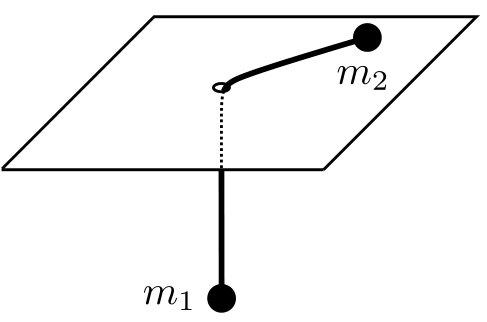
\includegraphics[width=0.3\textwidth]{content/Figures/2-2}
    \caption{ }
    \label{fig:2-2}
\end{figure}
\begin{solution}
    \begin{enumerate}[label=(\arabic*)]
        \item 设无约束时的广义坐标为$\{r_1, r_2, \theta\}$, 其中$r_1$和$r_2$分别是粒子与小孔之间的距离, $\theta$是粒子$m_2$在平面上运动的角度.
        约束方程为\[
            \phi (r_1, r_2, \theta) = r_1 + r_2 - l = 0
        \]
        注意到该约束方程是广义坐标的函数, 因此为完整约束; 且不显含时间, 因此为定常约束.
        \item 完整约束可减少一个自由度, 因此系统的自由度为$2$, 即最少只需两个独立的广义坐标$\{r, \theta\}$即可完全描述粒子的位形.
    \end{enumerate}
\end{solution}

\problem{如图\ref{fig:2-3}所示, 质量为$M$的楔块放在水平面上, 斜角分别为$\theta_1$和$\theta_2$, 底边长$L$. 两个质量分别为$m_1$和$m_2$的粒子, 
由一根无质量、不可拉伸的软绳连接, 绳长为$l$, 两个粒子分别放在楔块的两个斜面上. 不考虑摩擦, 
\begin{enumerate}[label=(\arabic*)]
    \item 分析楔块、两个粒子以及绳子组成的系统的位形与约束, 给出约束方程, 并分析约束是否完整、定常约束;
    \item 求系统的自由度.
\end{enumerate}}
\begin{figure}[h]
    \centering
    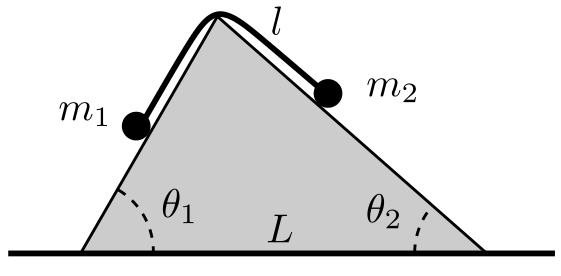
\includegraphics[width=0.3\textwidth]{content/Figures/2-3}
    \caption{ }
    \label{fig:2-3}
\end{figure}
\begin{solution}
    待施工.
\end{solution}


\setcounter{problem}{0}
\newpage
\chapter{相对论时空观}
\problem{考虑$2$维欧氏空间, 取一般坐标$\{u,v\}$, 与直角坐标关系为$x = x(u,v)$, $y = y(u,v)$. 求$2$维欧氏空间度规在$\{u,v\}$坐标下的形式.}
\begin{solution}
    由线元的定义, 我们有
    \begin{align*}
        \dd s^2 &= \left(\frac{\pp x}{\pp u} \dd u + \frac{\pp x}{\pp v} \dd v\right)^2 + \left(\frac{\pp y}{\pp u} \dd u + \frac{\pp y}{\pp v} \dd v\right)^2 \\
        &= \left(\frac{\pp x}{\pp u}\right)^2 \dd u^2 + \left(\frac{\pp x}{\pp v}\right)^2 \dd v^2 + \frac{\pp x}{\pp u} \frac{\pp x}{\pp v} \dd u \dd v + \left(\frac{\pp y}{\pp u}\right)^2 \dd u^2 + \left(\frac{\pp y}{\pp v}\right)^2 \dd v^2 + \frac{\pp y}{\pp u} \frac{\pp y}{\pp v} \dd u \dd v \\
        &= \begin{pmatrix}
            \dd u & \dd v
        \end{pmatrix} \begin{pmatrix}
            \left(\frac{\pp x}{\pp u}\right)^2 & \frac{\pp x}{\pp u} \frac{\pp x}{\pp v} \\[0.8em]
            \frac{\pp x}{\pp v} \frac{\pp y}{\pp u} & \left(\frac{\pp y}{\pp v}\right)^2
        \end{pmatrix} \begin{pmatrix}
            \dd u \\ \dd v
        \end{pmatrix}
    \end{align*}
    因此, 度规在$\{u,v\}$坐标下的形式为
    \[
        g_{ij} = \begin{pmatrix}
            \left(\frac{\pp x}{\pp u}\right)^2 & \frac{\pp x}{\pp u} \frac{\pp x}{\pp v} \\[0.8em]
            \frac{\pp x}{\pp v} \frac{\pp y}{\pp u} & \left(\frac{\pp y}{\pp v}\right)^2
        \end{pmatrix}
    \]
\end{solution}

\problem{考虑$3$维欧氏空间, 已知球坐标与直角坐标的关系为$x = r \sin\theta \cos\phi$, $y = r \sin\theta \sin\phi$, $z = r \cos\theta$. 求$3$维欧氏空间度规在球坐标下的形式.}
\begin{solution}
    考虑$3$维欧氏空间中的矢量$\vec{v} = x \h{x} + y \h{y} + z \h{z}$, 由球坐标$\begin{cases}
            x = r \sin\theta \cos\phi \\
            y = r \sin\theta \sin\phi \\
            z = r \cos\theta
        \end{cases}$
    构造坐标系的坐标基矢
    \[
        \begin{aligned}
            \frac{\pp \vec{v}}{\pp r} &= \sin\theta \cos\phi \,\h{x} + \sin\theta \sin\phi \,\h{y} + \cos\theta \,\h{z} \\
            \frac{\pp \vec{v}}{\pp \theta} &= r \cos\theta \cos\phi \,\h{x} + r \cos\theta \sin\phi \,\h{y} - r \sin\theta \,\h{z} \\
            \frac{\pp \vec{v}}{\pp \phi} &= -r \sin\theta \sin\phi \,\h{x} + r \sin\theta \sin\phi \,\h{y}
        \end{aligned}
    \]
    则线元可以写为
    \begin{align*}
        \dd s^2 &= \dd \vec{v} \cdot \dd \vec{v} = g_{ij} \dd u^i \dd u^j\\
        &= \begin{pmatrix}
            \dd r & \dd \theta & \dd \phi
        \end{pmatrix} \begin{pmatrix}
            g_{rr} & g_{r\theta} & g_{\theta\phi} \\
            g_{\theta r} & g_{\theta\theta} & g_{\theta\phi} \\
            g_{\phi r} & g_{\phi\theta} & g_{\phi\phi}
        \end{pmatrix} \begin{pmatrix}
            \dd r \\ \dd \theta \\ \dd \phi
        \end{pmatrix}
    \end{align*}
    其中$g_{ij} = g_{ji} = \frac{\pp \vec{v}}{\pp u^i} \cdot \frac{\pp \vec{v}}{\pp u^j} =
    \frac{\pp x}{\pp u^i} \frac{\pp x}{\pp u^j} + \frac{\pp y}{\pp u^i}
    \frac{\pp y}{\pp u^j} + \frac{\pp z}{\pp u^i} \frac{\pp z}{\pp u^j}$.
    
    \vspace*{1em}
    由于坐标基矢正交, 即非对角元为零, 计算对角元得
    \begin{align*}
        g_{rr} &= \left(\frac{\pp x}{\pp r}\right)^2 + \left(\frac{\pp y}{\pp r}\right)^2 + \left(\frac{\pp z}{\pp r}\right)^2 = (\sin \theta \cos \phi)^2 + (\sin \theta \sin \phi)^2 + (\cos \theta)^2 = 1, \\
        g_{\theta\theta} &= \left(\frac{\pp x}{\pp \theta}\right)^2 + \left(\frac{\pp y}{\pp \theta}\right)^2 + \left(\frac{\pp z}{\pp \theta}\right)^2 = (r \cos \theta \cos \phi)^2 + (r \cos \theta \sin \phi)^2 + (-r \sin \theta)^2 = r^2, \\
        g_{\phi\phi} &= \left(\frac{\pp x}{\pp \phi}\right)^2 + \left(\frac{\pp y}{\pp \phi}\right)^2 + \left(\frac{\pp z}{\pp \phi}\right)^2 = (-r \sin \theta \sin \phi)^2 + (r \sin \theta \cos \phi)^2 = r^2 \sin^2\theta.
    \end{align*}

    将$g_{ij}$代入线元, 得
    \[
        \dd s^2 = \begin{pmatrix}
            \dd r & \dd \theta & \dd \phi
        \end{pmatrix} \begin{pmatrix}
            1 & 0 & 0 \\
            0 & r^2 & 0 \\
            0 & 0 & r^2 \sin^2\theta
        \end{pmatrix} \begin{pmatrix}
            \dd r \\ \dd \theta \\ \dd \phi
        \end{pmatrix}
    \]
    即$3$维欧氏空间度规在球坐标下的形式为
    \[
        g_{ij} = \begin{pmatrix}
            1 & 0 & 0 \\
            0 & r^2 & 0 \\
            0 & 0 & r^2 \sin^2\theta
        \end{pmatrix}
    \]
\end{solution}


\problem{如图\ref{fig:3-3}所示, $2$维环面参数方程为 $\begin{cases}
    x = (R + r \cos \theta) \cos \phi, \\
    y = (R + r \cos \theta) \sin \phi, \\
    z = r \sin \theta
\end{cases}$, 其中 $R$ 和 $r$ 是常数, $\{\theta, \phi\}$ 为环面的坐标, 取值为 $0$ 到 $2\pi$. 求$2$维环面的度规.}
\begin{figure}[h]
    \centering
    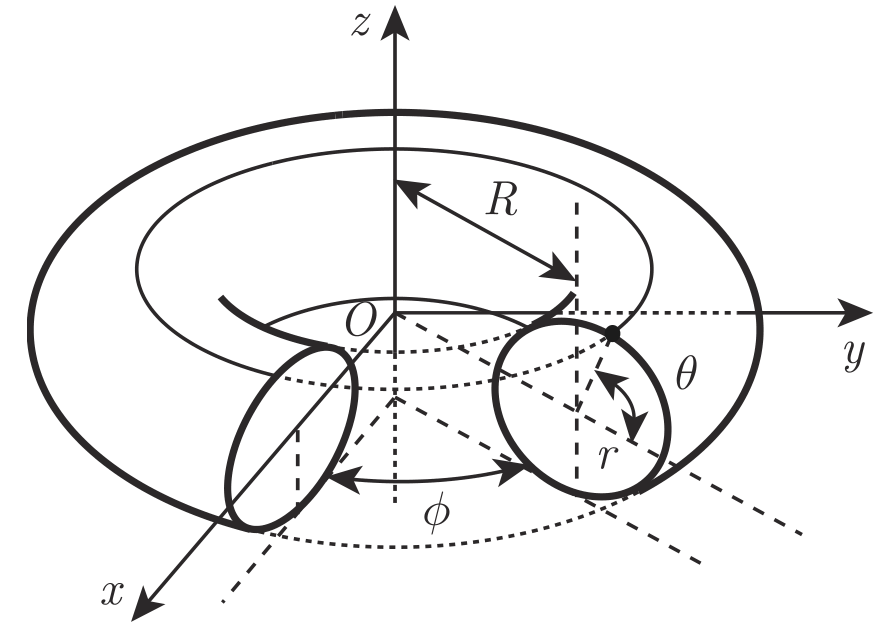
\includegraphics[width=0.3\textwidth]{content/Figures/3-3}
    \caption{ }
    \label{fig:3-3}
\end{figure}



\setcounter{problem}{0}
\newpage 
\chapter{最小作用量原理}

\problem{}
\begin{solution}
    待施工.
\end{solution}

\problem{}
\begin{solution}
    待施工.
\end{solution}


\problem{}
\begin{solution}
    待施工.
\end{solution}


\problem{}
\begin{solution}
    待施工.
\end{solution}


\problem{}
\begin{solution}
    待施工.
\end{solution}


\problem{}
\begin{solution}
    待施工.
\end{solution}


\problem{}
\begin{solution}
    待施工.
\end{solution}


\problem{}
\begin{solution}
    待施工.
\end{solution}



\problem{}
\begin{solution}
    待施工.
\end{solution}



\problem{}
\begin{solution}
    待施工.
\end{solution}



\problem{考虑与标量场相互作用的粒子作用量的 4 维形式和 3 维形式, 分别求粒子运动方程的 4 维形式和 3 维形式.}
\begin{solution}
    Minkowski 时空标量场中的粒子,其作用量为
    \[
        S = - m c \int \dd \tau \,\me^{\Phi} \sqrt{- \eta_{\mu \nu} \frac{\dd x^\mu}{\dd \tau} \frac{\dd x^\nu}{\dd \tau}},
    \]
    将被固有时 $\tau$ 参数化后的世界线 (作用量) 对 $x^\mu$ 作变分:
    \begin{align*}
        \delta S &= - mc \int \dd \tau \left[\frac{\pp}{\pp x^\mu} \left(\me^{\Phi} \sqrt{- \eta_{\mu \nu} \frac{\dd x^\mu}{\dd \tau} \frac{\dd x^\nu}{\dd \tau}}\right) \delta x^\mu + \frac{\pp}{\pp \left(\frac{\dd x^\mu}{\dd \tau}\right)} \left(\me^{\Phi} \sqrt{- \eta_{\mu \nu} \frac{\dd x^\mu}{\dd \tau} \frac{\dd x^\nu}{\dd \tau}}\right)\delta \left(\frac{\dd x^\mu}{\dd \tau}\right)\right]  \\
        &= - mc \int \dd \tau \left[\frac{\pp \Phi}{\pp x^\mu} \me^{\Phi} \sqrt{- \eta_{\mu \nu} \frac{\dd x^\mu}{\dd \tau} \frac{\dd x^\nu}{\dd \tau}} \delta x^\mu - \me^{\Phi} \frac{\eta_{\mu \nu} \frac{\dd x^\nu}{\dd \tau}}{\sqrt{- \eta_{\mu \nu} \frac{\dd x^\mu}{\dd \tau} \frac{\dd x^\nu}{\dd \tau}}} \delta \left(\frac{\dd x^\mu}{\dd \tau}\right)\right] \\
        & \simeq -mc \int \dd \tau \left[\frac{\pp \Phi}{\pp x^\mu} \me^{\Phi} \sqrt{- \eta_{\mu \nu} \frac{\dd x^\mu}{\dd \tau} \frac{\dd x^\nu}{\dd \tau}} + \frac{\dd}{\dd \tau} \left(\me^{\Phi} \frac{\eta_{\mu \nu} \frac{\dd x^\nu}{\dd \tau}}{\sqrt{- \eta_{\mu \nu} \frac{\dd x^\mu}{\dd \tau} \frac{\dd x^\nu}{\dd \tau}}}\right) \right] \delta x^\mu,
    \end{align*}
    因为 4-速度的模方是常数 $\eta_{\mu \nu} \frac{\dd x^\mu}{\dd \tau} \frac{\dd x^\nu}{\dd \tau} = - c^2$, 且由度规升降 $\eta_{\mu \nu} \frac{\dd x^\nu}{\dd \tau} \equiv \frac{\dd x_\mu}{\dd \tau}$, 所以我们可以写出 Euler-Lagrange 方程:
    \begin{align*}
        - \frac{1}{mc} \frac{\delta S}{\delta x^\mu} &= \frac{\pp \Phi}{\pp x^\mu} \me^\Phi c + \frac{\dd}{\dd \tau} \left(\frac{\me^\Phi}{c} \frac{\dd x_\mu}{\dd \tau}\right) = 0 \\
        &= c \frac{\pp \Phi}{\pp x^\mu} \me^\Phi + \frac{1}{c} \frac{\dd x_\mu}{\dd \tau} \frac{\pp \me^\Phi}{\pp \tau} + \frac{\me^\Phi}{c} \frac{\dd^2 x_\mu}{\dd \tau^2} = 0 \\
        &= c \frac{\pp \Phi}{\pp x^\mu} \me^\Phi + \frac{1}{c} \frac{\dd x_\mu}{\dd \tau} \frac{\pp x^\nu}{\pp \tau} \frac{\pp \Phi (x^\mu)}{\pp x^\nu} \me^\Phi + \frac{\me^\Phi}{c} \frac{\dd^2 x_\mu}{\dd \tau^2} = 0,
    \end{align*}
    即 4 维形式的运动方程
    \[
        \frac{\dd^2 x_\mu}{\dd \tau^2} + \frac{\pp \Phi}{\pp x^\nu} \frac{\pp x^\nu}{\pp \tau} \frac{\dd x_\mu}{\dd \tau} + c^2 \frac{\pp \Phi}{\pp x^\mu} = 0, \quad \mu = 0, 1, 2, 3.
    \]
    标量场作用下的作用量的 3 维形式为
    \[
        S = - m c \int \dd t\,\me^\Phi \sqrt{1- \frac{\delta_{ij}}{c^2} \frac{\dd x^i}{\dd t} \frac{\dd x^j}{\dd t}},
    \]
    对 3 维坐标 $x^i$ 作变分:
    \begin{align*}
        \delta S &= - mc \int \dd t \left[\frac{\pp}{\pp x^i} \left(\me^\Phi \sqrt{1- \frac{\delta_{ij}}{c^2} \frac{\dd x^i}{\dd t} \frac{\dd x^j}{\dd t}}\right) \delta x^i + \frac{\pp}{\pp \left(\frac{\dd x^i}{\dd t}\right)} \left(\me^\Phi \sqrt{1- \frac{\delta_{ij}}{c^2} \frac{\dd x^i}{\dd t} \frac{\dd x^j}{\dd t}}\right) \delta \left(\frac{\dd x^i}{\dd t}\right)\right] \\
        &= - mc \int \dd t \left[\frac{\pp \Phi}{\pp x^i} \me^\Phi \sqrt{1- \frac{\delta_{ij}}{c^2} \frac{\dd x^i}{\dd t} \frac{\dd x^j}{\dd t}} \delta x^i - \me^\Phi \frac{\delta_{ij} \frac{\dd x^j}{\dd t} \delta \left(\frac{\dd x^i}{\dd t}\right)}{c^2 \sqrt{1- \frac{\delta_{ij}}{c^2} \frac{\dd x^i}{\dd t} \frac{\dd x^j}{\dd t}}}\right] \\
        & \simeq - mc \int \dd t \left[\frac{\pp \Phi}{\pp x^i} e^\Phi \sqrt{1 - \frac{\vec{v}^2}{c^2}} + \frac{\dd}{\dd t} \left(\frac{\me^\Phi}{c^2} \frac{\frac{\dd x_i}{\dd t}}{\sqrt{1 - \frac{\vec{v}^2}{c^2}}}\right)\right] \delta  x^i, \\
        - \frac{\delta S}{\delta x^i} &= m c \frac{\pp \Phi}{\pp x^i} \me^\Phi \sqrt{1 - \frac{\vec{v}^2}{c^2}} + \frac{\me^\Phi}{c^2} \dot{\Phi} \frac{mc \frac{\dd x_i}{\dd t}}{\sqrt{1 - \frac{\vec{v}^2}{c^2}}} + \frac{\me^\Phi}{c^2} \frac{mc \frac{\dd^2 x_i}{\dd t^2}}{\sqrt{1 - \frac{\vec{v}^2}{c^2}}} = 0,
    \end{align*}
    3-动量定义为 $p_i \equiv m \frac{\dd x_i}{\dd t} \frac{\dd t}{\dd \tau} \equiv m \frac{\dd x_i}{\dd t} \frac{1}{\sqrt{1 - \frac{\vec{v}^2}{c^2}}}$, 则上式整理为, 
    \[
        \frac{\me^\Phi}{c} \left(\dot{\Phi} p_i + \dot{p}_i\right) + mc \frac{\pp \Phi}{\pp x^i} \me^\Phi \sqrt{1 - \frac{\vec{v}^2}{c^2}} = 0,
    \]
    即 3 维形式的运动方程
    \[
        \dot{p}_i + \dot{\Phi} p_i + mc^2 \sqrt{1 - \frac{\vec{v}^2}{c^2}} \frac{\pp \Phi}{\pp x^i} = 0, \quad i = 1, 2, 3.
    \]
\end{solution}



\problem{电磁场中带电粒子作用量的 4 维形式和 3 维形式分别为
    \begin{align*}
        S = \int \dd \tau L, \quad L = - m c \sqrt{- u_\mu u^\mu} + \frac{e}{c} A_\mu u^\mu, \\
        S = \int \dd \tau L, \quad L = - m c^2 \sqrt{1 - \frac{\vec{v}^2}{c^2}} - e \Phi + \frac{e}{c} \vec{v} \cdot \vec{A}.
    \end{align*}
    \begin{enumerate}[label=(\arabic*)]
        \item 求粒子的 4-共轭动量 $P_\mu \equiv \frac{\pp L}{\pp u^\mu}$ 和 3-共轭动量 $P_i \equiv \frac{\pp L}{\pp \dot{x}^i}$;
        \item 分别求粒子运动方程的 4 维形式和 3 维形式; 
        \item 若 $E$ 由式
        \[
            E := c p^0 = m c u^0 = m c^2 \frac{\dd t}{\dd \tau} = \frac{m c^2}{\sqrt{1 - \frac{\vec{v}^2}{c^2}}}
        \]
        给出, 证明 $\frac{\dd E}{\dd t} = e \vec{v} \cdot \vec{E}$.
    \end{enumerate}
}

\begin{solution}
    \begin{enumerate}[label=(\arabic*)]
        \item 待施工.
    \end{enumerate}
\end{solution}


\setcounter{problem}{0}
\newpage
\chapter{对称性与守恒律}

\problem{对于时间和广义坐标的任意函数\(F(t,\bm{q})\),证明其时间全导数\(\frac{\dd F}{\dd t}\)自动满足欧拉-拉格朗日方程,即其对应的运动方程恒为零。}

\begin{solution}
	证明只需作计算即可。记\(\dot{F}:=\frac{\dd F}{\dd t}\),那么
	\[\dot{F}=\frac{\dd F}{\dd t}=\frac{\partial F}{\partial t}+\frac{\partial F}{\partial q^a}\dot{q}^a\]
	计算
	\[\frac{\partial \dot{F}}{\partial q^a}=\frac{\partial^2 F}{\partial q^a\partial t}+\frac{\partial^2 F}{\partial q^a\partial q^b}\dot{q}^b\]
	\[\frac{\partial \dot{F}}{\partial \dot{q}^a}=\frac{\partial F}{\partial q^a}\]
	\[\frac{\dd}{\dd t}\frac{\partial \dot{F}}{\partial \dot{q}^a}=\frac{\partial^2 F}{\partial t\partial q^a}+\frac{\partial^2 F}{\partial q^a\partial q^b}\dot{q}^b\]
	考虑到偏导数可交换次序,可知
	\[\frac{\partial \dot{F}}{\partial q^a}-\frac{\dd}{\dd t}\frac{\partial \dot{F}}{\partial \dot{q}^a}=0\]
	恒成立,证毕。
	
	此题也可以从最小作用量原理来证明,将\(L=\frac{\dd F}{\dd t}\)代入得到
	\[S=\int_{t_1}^{t_2} L \dd t=\int_{t_1}^{t_2} \frac{\dd F}{\dd t} \dd t=F(t_2,\bm{q}(t_2))-F(t_1,\bm{q}(t_1))\]
	固定\(\bm{q}(t_1)\)和\(\bm{q}(t_2)\),那么上式右端是个常数,变分为零,自然满足欧拉-拉格朗日方程。
\end{solution}



\problem{单自由度系统的拉格朗日量为\(L=L(t,q,\dot{q})\)。(1)证明运动方程方程可以具体写成\(\frac{\partial^2 L}{\partial \dot{q}^2}\ddot{q}+\frac{\partial^2 L}{\partial q\partial \dot{q}}\dot{q}+\frac{\partial^2 L}{\partial t\partial \dot{q}}-\frac{\partial L}{\partial q}=0\);(2)若将\(L\)换成全导数\(\frac{\dd F}{\dd t}\),证明其自动满足(1)中的运动方程,即是恒等式。据此说明若两个拉格朗日量\(L\)和\(\tilde{L}\)相差时间全导数,即有\(\tilde{L}-L=\frac{\dd F}{\dd t}\),则给出相同的运动方程。}

\begin{solution}
	(1)欧拉-拉格朗日方程为
	\[\frac{\dd }{\dd t}\frac{\partial L}{\partial \dot{q}}-\frac{\partial L}{\partial q}=0\]
	使用链式法则即得
	\[\frac{\dd }{\dd t}\frac{\partial L}{\partial \dot{q}}=\frac{\partial^2 L}{\partial t\partial \dot{q}}+\frac{\partial^2 L}{\partial q\partial \dot{q}}\frac{\dd q}{\dd t}+\frac{\partial^2 L}{\partial \dot{q}^2}\frac{\dd \dot{q}}{\dd t}\]
	由于\(\frac{\dd q}{\dd t}=\dot{q},\frac{\dd \dot{q}}{\dd t}=\ddot{q}\),即得
	\[\frac{\partial^2 L}{\partial \dot{q}^2}\ddot{q}+\frac{\partial^2 L}{\partial q\partial \dot{q}}\dot{q}+\frac{\partial^2 L}{\partial t\partial \dot{q}}-\frac{\partial L}{\partial q}=0\]
	
	(2)证明在5.1题已经做过了,此处略。由此可知若\(\tilde{L}=L+\frac{\dd F}{\dd t}\),那么
	\[\frac{\partial \tilde{L}}{\partial q}-\frac{\dd }{\dd t}\frac{\partial \tilde{L}}{\partial \dot{q}}=\frac{\partial L}{\partial q}-\frac{\dd}{\dd t}\frac{\partial L}{\partial \dot{q}}+\frac{\partial \dot{F}}{\partial q}-\frac{\dd}{\dd t}\frac{\partial \dot{F}}{\partial \dot{q}}=\frac{\partial L}{\partial q}-\frac{\dd}{\dd t}\frac{\partial L}{\partial \dot{q}}\]
	也就是说,它们能给出相同的运动方程。
\end{solution}



\problem{某系统广义坐标为\(q\),已知其拉格朗日量为\(L=a\dot{q}^2+b\dot{q}^3\ddot{q}+c\ddot{q}q^3+d\ddot{q}\dot{q}q^2\),其中\(a,b,c,d\)都是常数。求与\(L\)相差时间全导数的、不含广义加速度\(\ddot{q}\)的等价拉格朗日量\(\tilde{L}\)。}

\begin{solution}
	推导只需反复分离全微分即可。
	
	对于\(a\dot{q}^2\)项,不含\(\ddot{q}\)。
	
	对于\(b\dot{q}^3\ddot{q}\)项,分部积分得到
	\[\dot{q}^3\ddot{q}=\frac{\dd }{\dd t}(\dot{q}^4)-3\dot{q}^3\ddot{q}\]
	即\(b\dot{q}^3\ddot{q}=\frac{1}{4}\frac{\dd }{\dd t}(b\dot{q}^4)\)。
	
	对于\(c\ddot{q}q^3\)项,分部积分得到
	\[\ddot{q}q^3=\frac{\dd}{\dd}(q^3 \dot{q})-3 q^2 \dot{q}^2\]
	即\(c\ddot{q}q^3=-3c q^2 \dot{q}^2+\frac{\dd}{\dd t}(c q^3 \dot{q})\)。
	
	对于\(d\ddot{q}\dot{q}q^2\)项,分部积分得到
	\begin{align*}
		\ddot{q}\dot{q}q^2&=\frac{\dd}{\dd t}(q^2 \dot{q}^2)-\dot{q}\frac{\dd}{\dd t}(q^2 \dot{q})\\
		&=-q^2\dot{q}\ddot{q}-2 q \dot{q}^3+\frac{\dd}{\dd t}(q^2 \dot{q}^2)\\
		2 \ddot{q}\dot{q}q^2&=-2 q \dot{q}^3+\frac{\dd}{\dd t}(q^2 \dot{q}^2)\\
		\ddot{q}\dot{q}q^2 &=-q \dot{q}^3+\frac{\dd}{\dd t}(\frac{1}{2}q^2 \dot{q}^2)
	\end{align*}
	即\(d\ddot{q}\dot{q}q^2=-d q \dot{q}^3+\frac{\dd}{\dd t}(\frac{1}{2}d q^2 \dot{q}^2)\)
	
	综合上述式子,得到
	\begin{align*}
		L&=a\dot{q}^2+b\dot{q}^3\ddot{q}+c\ddot{q}q^3+d\ddot{q}\dot{q}q^2\\
		&=a\dot{q}^2-3c q^2 \dot{q}^2-d q \dot{q}^3+\frac{\dd}{\dd t}(b\dot{q}^4+c q^3 \dot{q}+\frac{1}{2}d q^2 \dot{q}^2)
	\end{align*}
	与\(L\)相差时间全导数的、不含广义加速度\(\ddot{q}\)的等价拉格朗日量\(\tilde{L}\)为
	\[\tilde{L}=a\dot{q}^2-3c q^2 \dot{q}^2-d q \dot{q}^3\]
\end{solution}



\problem{已知质量\(m=1\)的一维谐振子拉格朗日量为\(L=\frac{1}{2}\dot{q}^2-\frac{1}{2}\omega^2 q^2\),考虑拉格朗日量\(\tilde{L}=\frac{1}{12}\dot{q}^4+\frac{\omega^2}{2}q^2 \dot{q}^2-\frac{\omega^4}{4}q^4\)。(1)证明\(L\)运动方程的解也是\(\tilde{L}\)的运动方程的解;(2)证明\(\tilde{L}\)不能表达成\(\tilde{L}=L+\frac{\dd F(t,q)}{\dd t}\)的形式。}

\begin{solution}
	(1)由欧拉-拉格朗日方程
	\[\frac{\partial L}{\partial q}-\frac{\dd}{\dd t}\frac{\partial L}{\partial \dot{q}}=0\]
	得到运动方程为\(\ddot{q}+\omega^2 q=0\)。对于\(\tilde{L}\)则为
	\[\frac{\partial \tilde{L}}{\partial q}-\frac{\dd}{\dd t}\frac{\partial \tilde{L}}{\partial \dot{q}}=0\]
	代入得到
	\[-\omega^4 q^3+\omega^2 q\dot{q}^2-\dot{q}^2\ddot{q}-\omega^2\frac{\dd }{\dd t}(q^2\dot{q})=0\]
	\[-\omega^4 q^3+\omega^2 q\dot{q}^2-\dot{q}^2\ddot{q}-\omega^2(q^2\ddot{q}+2q\dot{q}^2)=0\]
	整理为
	\[-\omega^2 q^2(\omega^2 q+\ddot{q})-\dot{q}^2(\omega^2 q+\ddot{q})=0\]
	\[-(\omega^2 q^2+\dot{q}^2)(\omega^2 q+\ddot{q})=0\]
	由于\(\omega^2 q^2+\dot{q}^2=0\)当且仅当\(q(t)=0\),此时\(q(t)\)同时满足两个方程,其余情况消去\(\omega^2 q^2+\dot{q}^2\),两个运动方程的解相同。
	
	(2)显然,由于
	\[\frac{\dd F(t,q)}{\dd t}=\frac{\partial F(t,q)}{\partial t}+\frac{\partial F(t,q)}{\partial q}\dot{q}\]
	其中只含有\(\dot{q}\)的一次项,但是\(\tilde{L}\)中含有\(\dot{q}\)的四次项,等式也就不能成立了。
\end{solution}



\problem{利用广义坐标和广义速度的变换关系,证明 (5.37)。}

\begin{solution}
	书中式(5.37)是如下的式子:
	\[\frac{\dd }{\dd t}\frac{\partial\tilde{L}}{\partial\dot{\tilde{q}}^a}-\frac{\partial\tilde{L}}{\partial \dot{\tilde{q}}^a}=\frac{\partial q^b}{\partial \tilde{q}^a}\left(\frac{\dd}{\dd t}\frac{\partial L}{\partial\dot{q}^b}-\frac{\partial L}{\partial q^b}\right)\]
	正文中给出了从最小作用量原理的推导过程,此处直接验证。
	
	待施工.
\end{solution}



\problem{已知一维谐振子的拉格朗日量为\(L=\frac{1}{2}m\dot{q}^2-\frac{1}{2}m\omega^2 q^2\),利用运动方程,证明\(C(t,q,\dot{q})=\arctan{\frac{\omega q}{\dot{q}}}-\omega t\)是运动常数。}

\begin{solution}
	由欧拉-拉格朗日方程得到运动方程为
	\[\ddot{q}+\omega^2 q=0\]
	对\(C(t,q,\dot{q})\)求导得到
	\[\frac{\dd C(t,q,\dot{q})}{\dd t}=\frac{\frac{\omega\dot{q}^2-\omega q \ddot{q}}{\dot{q}^2}}{1+\left(\frac{\omega q}{\dot{q}}\right)^2}-\omega=\frac{\omega\dot{q}^2-\omega q \ddot{q}}{\omega^2 q^2+\dot{q}^2}-\omega=\frac{\omega\dot{q}^2-\omega q \ddot{q}-\omega(\omega^2 q^2+\dot{q}^2)}{\omega^2 q^2+\dot{q}^2}=-\frac{\omega q(\ddot{q}+\omega^2 q)}{\omega^2 q^2+\dot{q}^2}=0\]
	因此\(C(t,q,\dot{q})=\arctan{\frac{\omega q}{\dot{q}}}-\omega t\)是运动常数,证毕。
\end{solution}



\problem{考虑例(2.9)中光滑细杆上的小球,如图\ref{fig:5-7}所示,假设细管放在光滑水平面上,且绕一端以恒定角速度\(\omega\)旋转。(1)选取合适的广义坐标,写出粒子的拉格朗日量并求其运动方程;(2)求粒子的能量函数\(h\),并分析其是否是运动常数;(3)粒子的能量函数\(h\)和总能量\(E=T+V\)相等吗?为什么?(4)粒子的总能量\(E=T+V\)是运动常数吗?尝试解释原因。}
\begin{figure}[h]
	\centering
	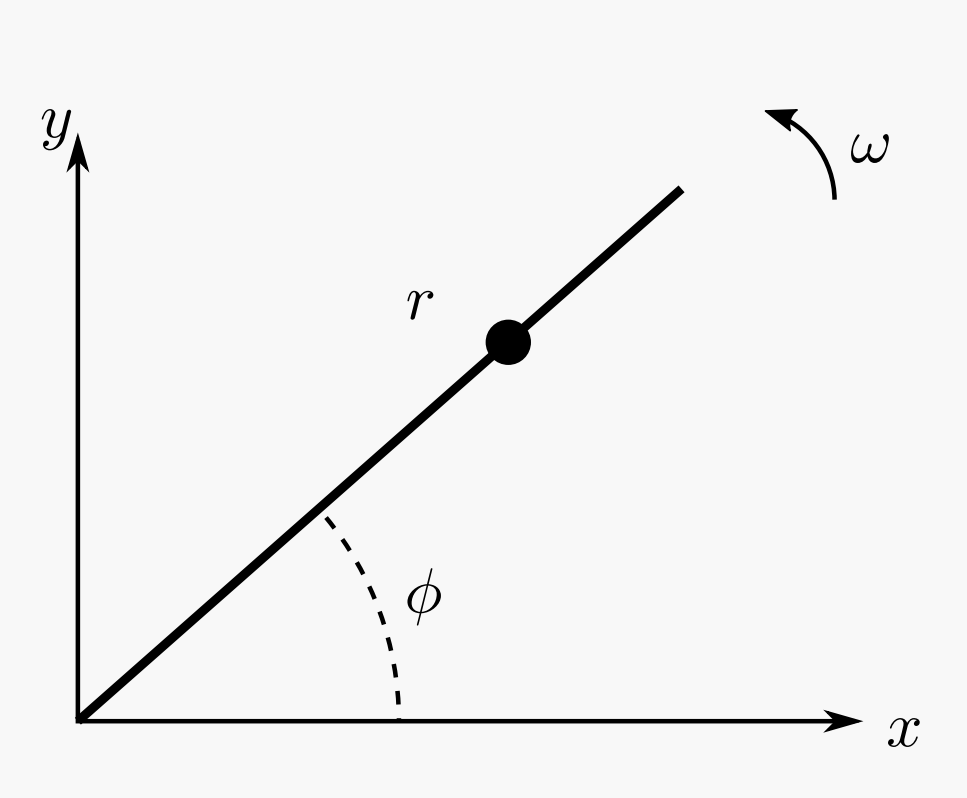
\includegraphics[width=0.3\textwidth]{content/Figures/5-7}
	\caption{ }
	\label{fig:5-7}
\end{figure}
	
\begin{solution}
	待施工.
\end{solution}



\problem{}
\begin{solution}
	待施工.
\end{solution}



\problem{}
\begin{solution}
	待施工.
\end{solution}



\problem{}
\begin{solution}
	待施工.
\end{solution}



\problem{}
\begin{solution}
	待施工.
\end{solution}



\problem{}
\begin{solution}
	待施工.
\end{solution}



\problem{}
\begin{solution}
	待施工.
\end{solution}



\problem{}
\begin{solution}
	待施工.
\end{solution}



\problem{}
\begin{solution}
	待施工.
\end{solution}



\problem{}
\begin{solution}
	待施工.
\end{solution}



\problem{}
\begin{solution}
	待施工.
\end{solution}




\setcounter{problem}{0}
\newpage 
\chapter{辅助变量}

\setcounter{problem}{0}
\newpage
\chapter{达朗贝尔原理}

\setcounter{problem}{0}
\newpage 
\chapter{两体问题}

\setcounter{problem}{0}
\newpage
\chapter{微扰展开}

\setcounter{problem}{0}
\newpage 
\chapter{小振动}
\problem{已知$n$个函数$\{u_1(t),\dots,u_n(t)\}$线性无关的“充分”条件是其朗斯基行列式 (Wronskian) 非零, 定义为
\[
    \mathcal{W}(u_1,\dots,u_n):=\det \begin{pmatrix}
        u_1 & u_2 & \cdots  & u_n\\
        u_1' & u_2' & \cdots & u_n'\\
        \vdots  & \vdots & \ddots & \vdots \\
        u_1^{(n-1)} & u_2^{(n-1)} & \cdots & u_n^{(n-1)} 
    \end{pmatrix}
\]其中$u^{(i)}$代表对$t$的$i$阶导数.
\begin{enumerate}[label=(\arabic*)]
    \item 证明$\me^{-\mi \omega t}$ 和其复共轭$\me^{+\mi \omega t}$是线性无关的, 即$\mathcal{W}(\me^{-\mi \omega t},\me^{+\mi \omega t})\neq 0$; 
    \item 证明任意复函数$u(t)$及其复共轭的朗斯基行列式$\mathcal{W}(u,u^\star)$只有虚部, 并讨论其非零的条件.
\end{enumerate}}
\begin{solution}
    \begin{enumerate}[label=(\arabic*)]
        \item 不难求得$\mathcal{W}(\me^{-\mi \omega t},\me^{+\mi \omega t})=2\mi \omega\neq 0$
        \item 对于任意复函数$u(t)$,
        \[
            \mathcal{W}(u, u^\star)=\det \begin{pmatrix}
                u & u^\star\\
                \dot{u} & \dot{u^\star}\\ 
            \end{pmatrix}
            =u\dot{u^\star}-(u\dot{u^\star})^\star
            =2\mathrm{Im}(u\dot{u^\star})    
        \]
        可见其只有虚部,非零要求$\mathrm{Im}(u\dot{u^\star})\neq 0$
    \end{enumerate}
\end{solution}

\problem{某单自由度系统, 广义坐标为$q$, 拉格朗日量为$L=\dfrac{1}{2}G(t)\dot{q}^2-\dfrac{1}{2}W(t)q^2$, 其中$G(t)$和$W(t)$都是时间的函数.
\begin{enumerate}[label=(\arabic*)]
    \item 若$q_1(t)$和$q_2(t)$为系统运动方程的任意两个线性无关的特解, 证明其朗斯基行列式$\mathcal{W}(t)=W(q_1(t),q_2(t))$满足形式为$\dot{\mathcal{W}}+f(t)\mathcal{W}=0$的微分方程, 并给出$f(t)$的表达式; 
    \item 根据 (1) 的结果, 分析当$G(t)$和$W(t)$满足什么条件时$\mathcal{W}$为常数.
\end{enumerate}}
\begin{solution}
    \begin{enumerate}[label=(\arabic*)]
        \item 易求得系统运动方程为
        \[
            G(t)\ddot{q}-\dot{G}(t)\dot{q}-W(t){q}=0
        \]
        转化为一阶常微分方程组为:
        \[
            \dot{\mathbf{q}}=\mathcal{A}(t)\mathbf{q}
        \]
        式中
        \[
            \mathcal{A}=\begin{pmatrix}
                0&1\\
                -W/G&-\dot{G}/G
            \end{pmatrix}
            ,\mathbf{q}=\begin{pmatrix}
                q&\dot{q}
            \end{pmatrix}^T
        \]
        现计算$\dot{\mathcal{W}}$.由线性常微分方程的Liouville定理,
        \[
            \dot{\mathcal{W}}=\mathrm{tr}(\mathcal{A})\mathcal{W}
        \]
        则$f(t)=-\mathrm{tr}(\mathcal{A})=\frac{\dot{G}(t)}{G(t)}$.
        \item 由于$\mathcal{W}\neq 0$,$\dot{\mathcal{W}}=0$意味着$\dot{G}(t)=0$
    \end{enumerate}
\end{solution}

\problem{待施工}
\begin{solution}
    待施工
\end{solution}

\problem{求习题9.5中系统做小振动的特征频率与简正模式, 并分析简正模式的物理意义.}
\begin{solution}
    待施工
\end{solution}

\problem{求习题9.6中系统做小振动的特征频率与简正模式, 并分析简正模式的物理意义.}
\begin{solution}
    待施工
\end{solution}

\problem{求习题9.7中系统做小振动的特征频率与简正模式, 并分析简正模式的物理意义.}
\begin{solution}
    待施工
\end{solution}

\setcounter{problem}{0}
\newpage
\chapter{转动理论}

\setcounter{problem}{0}
\newpage 
\chapter{刚体}
\problem{已知方阵的矩阵对数由$\ln({1+M})=M-\frac12M^2+\frac13M^3-\cdots$定义. 
    \begin{enumerate}[label=(\arabic*)]
        \item 给定同阶方阵$X,Y$, 证明矩阵指数$\me^{X}\me^{Y}=\me^{Z}$由所谓Baker-Campbell-Hausdorff公式给出, 即$Z=X+Y+\frac{1}{2}[X,Y]+\frac{1}{12}[X,[X,Y]]-\frac{1}{12}[Y,[X,Y]]+\cdots$. \label{prob:12.1.1}
        \item 仿照\ref{prob:12.1.1}的推导, 利用无穷小三维转动生成元的对易式求$\me^{-\psi J_3}\me^{-\theta J_1}\me^{-\phi J_3}=\me^{\phi^1J_1+\phi^2J_2+\phi^3J_3}$的$\phi^1,\phi^2,\phi^3$, 精确到2阶.
    \end{enumerate}
}
\begin{solution}
    \begin{enumerate}[label=(\arabic*)]
        \item 把$\me^{X},\me^{Y}$展开到3阶即可. 
            \begin{align*}
                \me^{X}\me^{Y}&=(1+X+\frac12X^2+\frac16X^3)(1+Y+\frac12Y^2+\frac16Y^3)\\&=
                1+X+\frac12X^2+\frac16X^3+Y+\frac12Y^2+\frac16Y^3+XY+\frac12X^2Y+\frac12XY^2
            \end{align*}
            \begin{align*}
                \ln(\me^{X}\me^{Y})&=X+Y+\frac12(X^2+Y^2+2XY)+\frac16(X^3+Y^3+3X^2Y+3XY^2+Y^3)-\\&\frac12(X+Y+\frac12(X^2+Y^2+2XY))^2+\frac13(X+Y)^3\\&=X+Y+\frac12(X^2+Y^2+2XY)+\frac16(X^3+Y^3+3X^2Y+3XY^2+Y^3)-\\&\frac12\Big(X^2+Y^2+XY+YX+\frac12((X+Y)(X^2+Y^2+2XY)+(X^2+Y^2+2XY)(X+Y))\Big)\\&+\frac13(X^3+Y^2X+XYX+YX^2+X^2Y+Y^3+XY^2+YXY)\\&=X+Y+\frac12(XY-YX)-\frac14(2X^3+2Y^3+2YXY+2XYX+3X^2Y+3XY^2+Y^2X+YX^2)\\&+\frac16(X^3+3X^2Y+3XY^2+Y^3)+\frac13(X^3+Y^2X+XYX+YX^2+X^2Y+Y^3+XY^2+YXY)\\&=X+Y+\frac{1}{2}[X,Y]+\frac{1}{12}[X,[X,Y]]-\frac{1}{12}[Y,[X,Y]]
            \end{align*}
        \item 要求是展开到2阶, 那么只需要取前两项. 
        根据SO(3)生成元之间的对易关系$[J_i,J_j]=\varepsilon_{ijk}J_k$
        $$\me^{-\psi J_3}\me^{-\theta J_1}=\me^{-\psi J_3+-\theta J_1+\frac12\psi\theta J_2}$$
        而
        \begin{align*}
            \me^{-\psi J_3}\me^{-\theta J_1}\me^{-\phi J_3}&=\me^{-\psi J_3-\theta J_1+\frac12\psi\theta J_2}\me^{-\phi J_3}\\&=\me^{-\psi J_3-\theta J_1+\frac12\psi\theta J_2-\phi J_3-\frac12[\psi J_3+\theta J_1-\frac12\psi\theta J_2, \phi J_3]}\\&=\me^{-\psi J_3-\theta J_1+\frac12\psi\theta J_2-\phi J_3-\frac12\theta\phi J_2}
        \end{align*}
        也就是说$\phi^1=-\theta,\phi^2=\frac{1}{2}(\psi-\phi)\theta,\phi^3=-\psi-\phi$.
    \end{enumerate}
\end{solution}

\problem{求质量为$m$的匀质椭球$\frac{x^2}{a^2}+\frac{y^2}{b^2}+\frac{z^2}{c^2}=1$的相对于质心的转动惯量张量}
\begin{solution}
    采用广义球坐标换元$x=ar\sin\theta\cos\phi=ax_1,y=br\sin\theta\sin\phi=by_1,z=cr\cos\theta=cz_1$, 则容易看出$r$从0变化到1, 且$r=1$时$x,y,z$满足椭球方程. 
    其体积元写为$\dd V=abcr^2\sin\theta\,\dd r\,\dd \theta\,\dd \phi=abc\,\dd x'\dd y'\dd z'$
    
    由于
    $$\int_{x_1^2+y_1^2+z_1^2\leq1}(x_1^2+y_1^2+z_1^2)\dd x_1\dd y_1\dd z_1=\int_{r_1^2\leq1}r_1^2\times r_1^2\dd r_1\times4\pi$$
    立刻得到
    $$\int_{r_1^2\leq1}x_1^2\dd x_1\dd y_1\dd z_1=\frac{4\pi}{15}$$
    由于球的密度$\rho=\frac{m}{\frac43\pi abc}$
    所以计算积分
    $$\int_{\frac{x^2}{a^2}+\frac{y^2}{b^2}+\frac{z^2}{c^2}\leq1}\rho x^2\dd x\,\dd y\,\dd z=\frac{3}{4\pi}a^2m\int_{r_1^2\leq1}x_1^2\dd x_1\dd y_1\dd z_1=\frac{1}{5}ma^2$$
    因此可以得到
    $$I_{xx}=\frac15m(b^2+c^2), I_{yy}=\frac15m(a^2+c^2), I_{zz}=\frac15m(a^2+b^2)$$
    非对角元都是0. 
\end{solution}
\problem{证明刚体惯量张量三个对角元中任意一个不会大于另外两个之和.}
\begin{solution}
    直接计算即可
    \begin{align*}
        I_{xx}+I_{yy}-I_{zz}&=\int \rho(y^2+z^2+x^2+z^2-x^2-y^2)\dd \tau\\&=2\int\rho z^2 \,\dd \tau\geq0
    \end{align*}
\end{solution}
\problem{考虑例12.4中的立方体. 
    \begin{enumerate}[label=(\arabic*)]
        \item 求其相对质心基矢垂直于立方体表面的本体系中惯量张量;
        \item 证明以质心为原点的任意本体坐标系均为其惯量主轴, 并由此说明当质心绕定点转动时, 匀质立方体和匀质球不可分辨.
    \end{enumerate}
}
\begin{solution}
    由于对称性可以知道其三个对角元素均为相同的, 而非对角元均为0, 仅计算一个即可
    $$I_{xx}=\int\frac{m}{a^3}(y^2+z^2)\dd x\,\dd y\,\dd z=\frac16ma^2$$
    由于其转动惯量张量写为
    $$\begin{pmatrix}
        \frac16ma^2&0&0\\
        0&\frac16ma^2&0\\
        0&0&\frac16ma^2
    \end{pmatrix}=\frac16ma^2\cdot I$$
    其中$I$是单位矩阵, 在正交变换下具有不变性
    $$I'=RIR^{-1}=RR^{-1}=I,$$
    因此其转动惯量张量在任何正交归一坐标系下形式不变, 也易知动能与绕质心转动球相同, 而动能一样运动自然一样. 
\end{solution}
\problem{求例11.5中圆盘相对于质心角动量在本体坐标系中分量形式}
\begin{solution}
    本体坐标系下角速度为
    $$\vec{\omega}=\omega\frac{R}{L}\cos\phi\,\h{e}_1+\omega\frac{R}{L}\sin\phi\,\h{e}_2-\omega\, \h{e}_3$$
    由于其转动惯量张量为
    $$\begin{pmatrix}
        \frac14mR^2&0&0\\0&\frac14mR^2&0\\0&0&\frac14mR^2
    \end{pmatrix}$$
    得到其角动量
    $$\vec{L}=\frac14m\omega\frac{R^3}{L}\cos\phi \,\h{e}_1+\frac{1}{4}m\omega\frac{R^3}{L}\sin\phi \,\h{e}_2-\frac12mR^2\omega\,\h{e}_3$$
\end{solution}
\problem{如图\ref{fig:12-14}所示, 一个宽为$l$高为$h$的门板绕着一边以角速度$\omega$匀速旋转, 建立如图的本体系$\{\h{e}_i\}$,
    \begin{enumerate}[label=(\arabic*)]
        \item 求门板相对于O点的角动量在$\{\h{e}_i\}$中的分量;
        \item 为了维持门的旋转, 需要施加的相对于O点的扭矩.
    \end{enumerate}}
\begin{figure}[h]
    \centering
    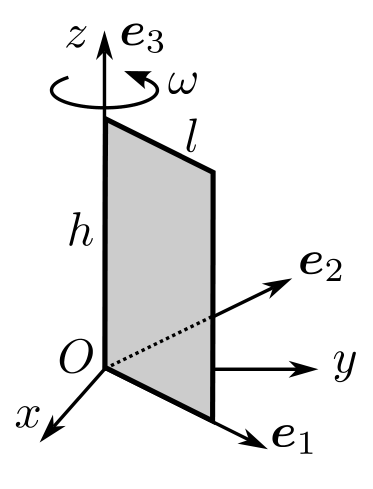
\includegraphics[width=0.2\textwidth]{content/Figures/12-14}
    \caption{ }
    \label{fig:12-14}
\end{figure}

\begin{solution}
    先求解相对于质心的角动量. 
    容易计算出其本体坐标系中的惯量张量为
    $$\begin{pmatrix}
        \frac{1}{12}mh^2&0&0\\0&\frac{1}{12}m(h^2+l^2)&0\\0&0&\frac{1}{12}ml^2
    \end{pmatrix}$$
    于是其相对于质心的角动量为
    $$\vec{L}_r=\frac{1}{12}ml^2\omega \,\h{e}_3$$
    再考虑质心相对于O点的角动量
    $$\vec{L}_c=m\vec{r}\times\vec{v}=\frac14m\omega l^2\,\h{e}_3-\frac14m\omega hl\,\h{e}_1$$
    熟知相对于O点角动量等于两项之和
    $$\vec{L}=\frac13m\omega l^2\,\h{e}_3-\frac14m\omega hl\,\h{e}_1$$
    当然可以直接计算其相对于O点的惯量张量. 
    $$I_{11}=\frac13mh^2,I_{22}=\frac13m(h^2+l^2),I_33=\frac13mh^2$$
    以及
    $$I_{13}=I_{31}=-\int\rho xz\dd x\,\dd z=-\frac14mhl$$
    再利用角动量公式$\vec{L}=\vec{I}\vec{\omega}$得到一样的结果. 
    由熟知公式
    $$\Big(\frac{\dd}{\dd t}\Big)_{\text{space}}=\Big(\frac{\dd}{\dd t}\Big)_{\text{body}}+\vec{\omega}\times$$
    得到力矩
    $$\vec{M}=\vec{\omega}\times\vec{L}=\frac14mhl\omega^2$$
\end{solution}
\problem{若自由刚体定点转动的角速度沿着某个主轴方向, 则被称为匀速转动. 
    \begin{enumerate}[label=(\arabic*)]
        \item 证明任意自由刚体都有匀速转动解;
        \item 设初始角速度沿着$\h{e}_1$方向, 刚体收到小扰动, 角速度变为$\omega_i\to\omega_i+\delta\omega_i$,求$\delta\omega_i$满足的微分方程并写成小振动方程的形式. \label{prob:12.7.2}
        \item 设刚体的主轴转动惯量为$I_1<I_2<I_3$, 利用\ref{prob:12.7.2}的结果, 证明刚体沿着最小和最大转动惯量对应的主轴的匀速转动是稳定的, 而沿着中间转动惯量对应的主轴的转动是不稳定的.
    \end{enumerate}}
\begin{solution}
    \begin{enumerate}[label=(\arabic*)]
        \item 只需要$\omega_1=C,\omega_2=\omega_3=0$或与其类似即可满足欧拉动力学方程.
        \item 由题知道角速度为
        $$\vec{\omega}=(\omega_1+\delta\omega_1)\,\h{e}_1+\delta\omega_2\,\h{e}_2+\delta\omega_3\,\h{e}_3$$
        由自由转动时三个欧拉动力学方程
        \begin{align*}
            I_1\dot{\delta\omega_1}&=\delta\omega_2\delta\omega_3(I_2-I_3)\\
            I_2\dot{\delta\omega_2}&=\delta\omega_3(\omega_1+\delta\omega_1)(I_3-I_1)\\
            I_3\dot{\delta\omega_3}&=(\omega_1+\delta\omega_1)\delta\omega_2(I_1-I_2)
        \end{align*}
        知道, 由于$\delta\omega_2,\delta\omega_3$都是小量, $\delta\omega_1$可以忽略. 
        因此原运动方程化为2元的
        \begin{align}
            I_2\dot{\delta\omega_2}&=\delta\omega_3\omega_1(I_3-I_1)\\
            I_3\dot{\delta\omega_3}&=\omega_1\delta\omega_2(I_1-I_2)
        \end{align}
        在(2)两边求导后带入(1)得到关于$\delta\omega_3$的二阶线性微分方程
        $$\ddot{\delta\omega_3}+\frac{(I_2-I_1)(I_3-I_1)}{I_2I_3}\omega_1^2\delta\omega_3=0$$
        同样可以得到
        $$\ddot{\delta\omega_2}+\frac{(I_2-I_1)(I_3-I_1)}{I_2I_3}\omega_1^2\delta\omega_2=0$$
        其假如存在小振动解, 本征频率为$\Omega=\sqrt{\frac{(I_2-I_1)(I_3-I_1)}{I_2I_3}}\omega_1$
        \item 假如初始绕着$2$轴旋转, 知道其本征频率为$\Omega=\sqrt{\frac{(I_1-I_2)(I_3-I_2)}{I_1I_3}}\omega_2$
        但是$I_1<I_2<I_3$, 所以根号下小于$0$, 对应解指数发散, 即不稳定.
    \end{enumerate}
\end{solution}

\problem{设对称陀螺相对质心的主轴转动惯量为$I_1=I_2=\lambda I_3$, 若陀螺绕质心自由转动, 初始章动角为$\theta_0$, 证明进动角速度$\dot{\psi}$与自转角速度$\dot{\varphi}$满足$\dot\psi=(\lambda-1)\dot\phi\cos\theta_0$}
\begin{solution}
    这题还是用欧拉动力学方程. 
    由于$I_1=I_2$, 立刻得到$\omega_3=C$
    由此得到关于$\omega_1,\omega_2$的方程
    \begin{align*}
        \lambda\dot{\omega_1}&=\omega_2\omega_3(\lambda-1)\\
        \lambda\dot{\omega_2}&=\omega_2\omega_3(-\lambda+1)
    \end{align*}
    因此解得
    $$\omega_1=A\cos(\frac{\lambda-1}{\lambda}\omega_3 t+\varphi),\omega_1=A\sin(\frac{\lambda-1}{\lambda}\omega_3 t+\varphi)$$
    也就是说, 有守恒量$\omega_1^2+\omega_2^2=C$
    于是可以知道总角动量大小守恒, 因为
    $$L^2=\lambda^2 I_3^2(\omega_1^2+\omega_2^2)+I_3^2\omega_3^2$$
    正文中已经给出, z轴角动量分量$p_\psi$也守恒, 即
    $$\cos\theta=\frac{p_\psi}{L}=\cos\theta_0$$
    为常数!
    由欧拉运动学方程得到
    $$\omega_1^2+\omega_2^2=\sin^2\theta\dot\phi^2+\dot\theta^2=C'$$
    即$\dot\phi=\frac{A}{\sin\theta_0}$是一个常数
    
    但是由于$$L^2=\lambda^2I_3^2(\omega_1^2+\omega_2^2)+I_3^2\omega_3^2=\lambda^2 I_3^2(\omega_1^2+\omega_2^2)+L^2\cos^2\theta$$
    于是可以得到
    $$\dot\phi=\frac{L}{\lambda I_3}$$
    由于$p_\psi=L\cos\theta=I_3(\dot\psi+\dot\phi\cos\theta_0)$
    解得
    $$\dot\psi=\frac{L(\lambda-1)}{I_3\lambda}\cos\theta_0$$
    即得到题给式子
    $$\dot\psi=(\lambda-1)\dot\phi\cos\theta_0$$
\end{solution}


\setcounter{problem}{0}
\newpage
\chapter{哈密顿正则方程}
\problem{求二元函数$L=ax^2+2bxy+cy^2+dx+ey$的对$x,y$的勒让德变换.}
\begin{solution}
    \begin{align*}
        H&=\sum\frac{\partial L}{\partial x_i}x_i-L\\&=ax^2+2bxy+cy^2
    \end{align*}
\end{solution}
\problem{考虑函数$L=\frac12(q^1v^2-q^2v^1)-V(q^1,q^2)$,其中$\{q^1,q^2\}$为被动变量,$\{v^1,v^2\}$为主动变量,$V$是任意函数.
\begin{enumerate}[label=(\arabic*)]
\item 分析$L$对$\{v^1,v^2\}$的黑塞矩阵,判断其是奇异还是正规系统;\item 定义新变量$p_1=\frac{\partial L}{\partial v^1},p_2\frac{\partial L}{\partial v^2}$,求$\{q^1,q^2,p^1,p^2\}$之间的约束关系.
\end{enumerate}}
\begin{solution}
\begin{enumerate}[label=(\arabic*)]
    \item 黑塞矩阵为
    $$\Big(\frac{\partial^2 L}{\partial v^{i}\partial v^{j}}\Big)=\begin{pmatrix}
        0&0\\0&0
    \end{pmatrix}$$
    显然为奇异系统。

    \item $$p_1=\frac12q^1,p_2=-\frac12q^2$$
    这就是约束关系。
\end{enumerate}
\end{solution}
\problem{考虑例4.4中的双摆,求系统的哈密顿量和哈密顿正则方程.}
\begin{solution}
    由正文得到
    $$L=\frac{1}{2}(m_1+m_2)l_1^2\dot \theta_1^2+\frac12m_2l_2^2\dot \theta_2^2+m_2l_1l_2\dot \theta_1\dot \theta_2\cos(\theta_1-\theta_2)+m_1gl_1\cos\theta_1+m_2g(l_1\cos\theta_1+l_2\cos\theta_2)$$
    由广义动量的定义
    \begin{align*}
        p_1&=\frac{\partial L}{\partial \dot\theta_1}=(m_1+m_2)l_1^2\dot\theta_1+m_2l_1l_2\dot\theta_2\cos(\theta_1-\theta_2)\\
        p_2&=\frac{\partial L}{\partial \dot\theta_2}=m_2l_2^2\dot\theta_2++m_2l_1l_2\dot\theta_1\cos(\theta_1-\theta_2)
    \end{align*}
    解得
    \begin{align*}
        \dot\theta_1&=\frac{p_1-\frac{l_1}{l_2}p_2}{m_1l_1^2+m_2l_1^2(1-\cos^2(\theta_1-\theta_2))}\\
        \dot\theta_2&=\frac{\frac{(m_1+m_2)l_1}{m_2l_2}p_2-\cos(\theta_1-\theta_2)p_1}{m_1l_1+m_2l_1(1-\cos^2(\theta_1-\theta_2))}
    \end{align*}
    代入哈密顿量表达式得到
    \begin{align*}
        H&=\sum_{i}p_{i}\dot\theta_i-L\\
         &=\frac{1}{2}(m_1+m_2)l_1^2\dot \theta_1^2+\frac12m_2l_2^2\dot \theta_2^2+m_2l_1l_2\dot \theta_1\dot \theta_2\cos(\theta_1-\theta_2)-m_1gl_1\cos\theta_1-m_2g(l_1\cos\theta_1+l_2\cos\theta_2)\\
         &=\frac12p_1\dot\theta_1+\frac12p_2\dot\theta_2-m_1gl_1\cos\theta_1-m_2g(l_1\cos\theta_1+l_2\cos\theta_2)\\
         &=\frac{p_1^2-(\frac{l_1}{l_2}+\cos(\theta_1-\theta_2))p_1p_2+(1+\frac{m_1}{m_2})\frac{l_1}{l_2}p_2^2}{2l_1^2(m_1+m_2\sin^2(\theta_1-\theta_2))}-m_1gl_1\cos\theta_1-m_2g(l_1\cos\theta_1+l_2\cos\theta_2)
    \end{align*}
    正则方程
    \begin{align*}
        \dot\theta_1&=\frac{p_1-(\frac{l_1}{l_2}+\cos(\theta_1-\theta_2))p_2}{l_1^2(m_1+m_2\sin^2(\theta_1-\theta_2))}\\
        \dot\theta_2&=\frac{-(\frac{l_1}{l_2}+\cos(\theta_1-\theta_2))p_1+(1+\frac{m_1}{m_2})\frac{l_1}{l_2}p_2}{l_1^2(m_1+m_2\sin^2(\theta_1-\theta_2))}\\
        \dot p_1&=-\frac{2p_1p_2\sin(\theta_1-\theta_2)l_1^2(m_1+m_2\sin^2(\theta_1-\theta_2))}{4l_1^4(m_1+m_2\sin^2(\theta_1-\theta_2))^4}\\
        &-\frac{2m_2\sin(\theta_1-\theta_2)\cos(\theta_1-\theta_2)(p_1^2-(\frac{l_1}{l_2}+\cos(\theta_1-\theta_2))p_1p_2+(1+\frac{m_1}{m_2})\frac{l_1}{l_2}p_2^2)}{4l_1^4(m_1+m_2\sin^2(\theta_1-\theta_2))^4}\\
        &-(m_1+m_2)gl_1\sin\theta_1\\
        \dot p_2&=-\frac{2p_1p_2\sin(\theta_1-\theta_2)l_1^2(m_1+m_2\sin^2(\theta_1-\theta_2))}{4l_1^4(m_1+m_2\sin^2(\theta_1-\theta_2))^4}\\
        &-\frac{2m_2\sin(\theta_1-\theta_2)\cos(\theta_1-\theta_2)(p_1^2-(\frac{l_1}{l_2}+\cos(\theta_1-\theta_2))p_1p_2+(1+\frac{m_1}{m_2})\frac{l_1}{l_2}p_2^2)}{4l_1^4(m_1+m_2\sin^2(\theta_1-\theta_2))^4}\\
        &-m_2gl_2\sin\theta_2
    \end{align*}
\end{solution}
\problem{考虑例4.5中的顶端自由滑动的单摆,求系统的哈密顿量和哈密顿正则方程.}
\begin{solution}
    解得
    \begin{align*}
        p_x&=m\dot x+ml\dot\theta\cos\theta\\
        p_\theta&=ml^2\dot \theta+m\dot xl\cos\theta
    \end{align*}
    反解得到
    \begin{align*}
        \dot x&=\frac{lp_x-p_\theta\cos\theta}{ml\sin^2\theta}\\
        \dot \theta&=\frac{p_\theta-p_xl\cos\theta}{ml^2}
    \end{align*}
    \begin{align*}
        H&=\sum p_iq^i-L\\
         &=\frac12\Big(\dot x(\dot x+l\dot\theta\cos\theta)+l\dot\theta(l\dot\theta+\dot x\cos\theta)\Big)-mgl\cos\theta\\
         &=\frac12p_x\dot x+\frac12p_\theta\dot\theta-mgl\cos\theta\\
         &=\frac12p_x\frac{lp_x-p_\theta\cos\theta}{ml\sin^2\theta}+\frac12p_\theta\frac{p_\theta-p_xl\cos\theta}{ml^2}-mgl\cos\theta\\
         &=\frac{p_x^2}{2m\sin^2(\theta)}-\frac{p_xp_\theta}{2ml}\cos\theta(\frac{1}{\sin^2\theta}+1)+\frac{p_\theta^2}{2ml^2}
    \end{align*}
    哈密顿正则方程
    \begin{align*}
        \dot x&=\frac{p_x}{m\sin^2\theta}-\frac{p_\theta}{2ml}\cos\theta(\frac{1}{\sin^2\theta}+1)\\
        \dot\theta&=-\frac{p_\theta}{2ml}\cos\theta(\frac{1}{\sin^2\theta}+1)+\frac{p_\theta}{ml^2}\\
        \dot p_x&=0\\
        \dot p_\theta&=\frac{p_x^2}{m\sin^3\theta}\cos\theta-\frac{p_xp_\theta}{2ml}\sin\theta-\frac{p_xp_\theta\cos^2\theta}{\sin^3\theta}
    \end{align*}
\end{solution}
\problem{已知系统的广义坐标为$L=a\dot x^2+b\frac{\dot y^2}{x}+c\dot x\dot y+fy^2\dot x\dot z+g\dot y^2-k\sqrt{x^2+y^2}$,其中$a,b,c,d,f,g,k$都是常数.
\begin{enumerate}[label=(\arabic*)]
    \item 求系统的哈密顿量和哈密顿正则方程.
    \item 求系统的运动常数.
\end{enumerate}}
\begin{solution}
    \begin{enumerate}[label=(\arabic*)]
    \item 系统广义动量
    \begin{align*}
        p_x&=2a\dot x+c\dot y+fy^2\dot z\\
        p_y&=\frac{2b\dot y}{x}+c\dot x+2g\dot y\\
        p_z&=fy^2\dot x
    \end{align*}
    反解得到
    \begin{align*}
        \dot x&=\frac{p_z}{fy^2}\\
        \dot y&=\frac{p_y-\frac{cp_z}{fy^2}}{\frac{2b}{x}+2g}\\
        \dot z&=\frac{(p_x-\frac{2ap_z}{fy^2})(\frac{2b}{x}+2g)-cp_y+\frac{c^2p_z}{fy^2}}{fy^2(\frac{2b}{x}+2g)}
    \end{align*}
    哈密顿量
    \begin{align*}
        H&=\sum_{i}p_i\dot x^i-L\\&=2a\dot x^2+c\dot y\dot x+fy^2\dot z\dot x+\frac{2b\dot y^2}{x}+c\dot x\dot y+2g\dot y^2+fy^2\dot x\dot z\\&-(a\dot x^2+b\frac{\dot y^2}{x}+c\dot x\dot y+fy^2\dot x\dot z+g\dot y^2-k\sqrt{x^2+y^2})\\&=a\dot x^2+c\dot x\dot y+fy^2\dot x\dot z+g\dot y^2+\frac{b\dot y^2}{x}+k\sqrt{x^2+y^2}\\&=a\frac{p_z^2}{f^2y^4}+c\frac{p_z}{fy^2}\frac{p_y-\frac{cp_z}{fy^2}}{\frac{2b}{x}+2g}+p_z\frac{(p_x-\frac{2ap_z}{fy^2})(\frac{2b}{x}+2g)-cp_y+\frac{c^2p_z}{fy^2}}{fy^2(\frac{2b}{x}+2g)}\\&+g\frac{(p_y-\frac{cp_z}{fy^2})^2}{2(\frac{2b}{x}+2g)}+k\sqrt{x^2+y^2}\\&=-a\frac{p_z^2}{f^2y^4}+\frac{p_xp_z}{fy^2}+g\frac{(p_y-\frac{cp_z}{fy^2})^2}{2(\frac{2b}{x}+2g)}+k\sqrt{x^2+y^2}
    \end{align*}
    由哈密顿正则方程
    \begin{align*}
        \dot x&=\frac{\partial H}{\partial p_x}=\frac{p_z}{fy^2}\\
        \dot y&=\frac{\partial H}{\partial p_y}=\frac{g(p_y-\frac{cp_z}{fy^2})}{\frac{2b}{x}+2g}\\
        \dot z&=\frac{\partial H}{\partial p_z}=-\frac{2ap_z}{f^2y^4}+\frac{p_x}{fy^2}+\frac{gc(p_y-\frac{cp_z}{fy^2})}{(\frac{2b}{x}+2g)fy^2}\\
        \dot p_x&=-\frac{\partial H}{\partial x}=--\frac{b(p_y-\frac{cp_z}{fy^2})^2}{4(b+gx)^2}-\frac{kx}{\sqrt{x^2+y^2}}\\
        \dot p_y&=-\frac{\partial H}{\partial y}=-\frac{4p_z^2}{f^2y^5}(4a-\frac{gc^2}{4(\frac bx+g)})-\frac{2p_z}{fy^3}(p_x-\frac{gcp_y}{2(\frac{b}{x}+g)})\\
        \dot p_z&=0
    \end{align*}
    \item 可以知道$p_z,H$是守恒量。
    \end{enumerate}
\end{solution}
\problem{某单自由度系统的运动方程为$\dot q=q^2+qp,\dot p=p^2-qp$,利用(13.29)判断其是否为哈密顿系统.}
\begin{solution}
    由正文得到
    \begin{align*}
        u&=q^2+qp\\
        v&=p^2-qp\\
    \end{align*}
    计算得到
    \begin{align*}
        &\frac{\partial u}{\partial q}=2q+p,\frac{\partial u}{\partial p}=q\\
        &\frac{\partial v}{\partial q}=-p,\frac{\partial v}{\partial p}=2p-q\\
    \end{align*}
    明显不满足$\frac{\partial u}{\partial q}=-\frac{\partial v}{\partial p}$,不是哈密顿系统.
\end{solution}
\problem{某单自由度系统运动方程为$\dot q=p$和$\dot p=-\omega^2 q-2\lambda p$,其中$\omega$和$\lambda$都是常数;
\begin{enumerate}[label=(\arabic*)]
    \item 利用(13.29)判断其是否为哈密顿系统;
    \item 引入新变量$Q=q$和$P=p\me^{2\lambda t}$,求$Q$和$P$的运动方程,判断其是否为哈密顿系统并求哈密顿量.
\end{enumerate}}
\begin{solution}
    \begin{enumerate}[label=(\arabic*)]
        \item \begin{align*}
            &\frac{\partial u}{\partial q}=0\\
            &\frac{\partial v}{\partial p}=-2\\
              \end{align*}
        显然不是
        \item 由题设易知道$\dot p+2\lambda p=\dot P \me^{-2\lambda t}$
        于是其运动方程写为
        \begin{align*}
            \dot Q&=P\me^{-2\lambda t}\\
            \dot P&=-\omega^2 Q\me^{2\lambda t}
        \end{align*}
        此时$\frac{\partial u}{\partial Q}=\frac{\partial v}{\partial P}=0$满足哈密顿系统的微分条件

        由哈密顿方程得到
        \begin{align*}
            \frac{\partial H}{\partial P}&=P\me^{-2\lambda t}\\
            \frac{\partial H}{\partial Q}&=\omega^2 Q\me^{2\lambda t}
        \end{align*}
        于是,由全微分条件得到
        $$H=\frac12 Q^2\me^{2\lambda t}+\frac12 P^2\me^{-2\lambda t}$$
    \end{enumerate}
\end{solution}
\problem{某单自由度系统的运动方程为$\dot q=aq+bp$和$\dot p=cq+dp$
\begin{enumerate}[label=(\arabic*)]
    \item 利用(13.29)判断$a,b,c,d$满足什么条件时,系统为哈密顿系统;
    \item 求对应的哈密顿量.
\end{enumerate}}
\begin{solution}
    \begin{enumerate}[label=(\arabic*)]
        \item 由正文得到
        \begin{align*}
            &\frac{\partial u}{\partial q}=a\\
            &\frac{\partial v}{\partial p}=d\\
        \end{align*}
        要求满足$a=-d$即可;
        \item 由上一题得到
        \begin{align*}
            \frac{\partial H}{\partial p}&=aq+bp\\
            \frac{\partial H}{\partial q}&=ap-cq
        \end{align*}
        由$H=H(q,p)$的全微分条件
        \begin{align*}
            dH&=\frac{\partial H}{\partial p}dp+\frac{\partial H}{\partial q}dq\\
              &=(aq+bp)dp+(ap-cq)dq\\
              &=-cqdq+a(qdp+pdq)+apdp\\
              &=-cqdq+ad(pq)+apdp
        \end{align*}
        积分即得到
        $$H=-\frac12 cq^2+apq+\frac12 p^2$$
    \end{enumerate}
\end{solution}
\problem{考虑与标量场相互作用的相对论性粒子的拉格朗日量式(4.40),其中$\Phi(t,\textbf{x})=\frac{V(t,\textbf{x})}{mc^2}$.
\begin{enumerate}[label=(\arabic*)]
    \item 求粒子的哈密顿量和正则方程;
    \item 求非相对论极限下哈密顿量的领头阶近似.
\end{enumerate}}
\begin{solution}
由于我的习惯,本题采用约定
$$(\eta_{\mu\nu})=
    \begin{pmatrix}
    1&0&0&0\\
    0&-1&0&0\\
    0&0&-1&0\\
    0&0&0&-1
    \end{pmatrix}$$
    \begin{enumerate}[label=(\arabic*)]
    \item 我们考虑三维形式的拉格朗日量和哈密顿量,由相对论性点粒子与标量场耦合的作用量
    $$S=-\int mc\me^{\Phi}ds=-\int mc\me^{\Phi}\frac{ds}{dt}dt=$$
    并且考虑到$ds^2=dt^2-dx^2-dy^2-dz^2=dt^2(1-\frac{v^2}{c^2})$
    得到三维拉格朗日量$$L=-mc^2\sqrt{1-\frac{v^2}{c^2}}\me^{\Phi}$$
    以及广义动量
    $$\textbf{p}=\frac{\partial L}{\partial \textbf{v}}=\frac{m\textbf{v}\me^{\Phi}}{\sqrt{1-\frac{v^2}{c^2}}}$$
    反解得到
    $$\textbf{v}=\frac{\textbf{pc}}{\sqrt{m^2c^2\me^{2\Phi}+p^2}}$$
    最后得到哈密顿量
    $$H=\textbf{p}\cdot{\textbf{v}}-L=\sqrt{p^2c^2+m^2c^4\me^{2\Phi}}$$
    而前面已经得到了一个正则方程
    $$\textbf{v}=\frac{\textbf{pc}}{\sqrt{m^2c^2\me^{2\Phi}+p^2}}$$
    因此我们只需要考虑$\frac{d\textbf{p}}{dt}=-\frac{\partial H}{\partial \textbf{x}}$
    经过计算得到
    $$\frac{d\textbf{p}}{dt}=-\frac{m^2c^4\me^{2\Phi}}{\sqrt{p^2c^2+m^2c^4\me^{2\Phi}}}\nabla\Phi$$
    \item 
    \begin{align*}
        H&=mc^2\me^{\Phi}\sqrt{\frac{p^2}{m^2c^2\me{2\Phi}}+1}\\
         &=mc^2\me^{\Phi}(1+\frac{p^2}{2m^2c^2\me{2\Phi}})\\
         &=mc^2(1+\frac{V}{mc^2})(1+\frac{p^2}{2m^2c^2\me^{2\Phi}})\\
         &=mc^2+\frac12mv^2+V
    \end{align*}
    \end{enumerate}
\end{solution}
\problem{考虑电磁场中相对论性带电粒子的拉格朗日量式(4.50).
\begin{enumerate}[label=(\arabic*)]
    \item 求粒子的哈密顿量和哈密顿正则方程;
    \item 由哈密顿正则方程得到等价的关于$\textbf{x}$的二阶微分方程;
    \item 求非相对论极限下哈密顿量的领头阶近似.
\end{enumerate}
}
\begin{solution}
    \begin{enumerate}[label=(\arabic*)]
    先考虑正文中提及的三维形式
        \item $$L=-mc^2\sqrt{1-\frac{v^2}{c^2}}-q\varphi+q\textbf{v}\cdot\textbf{A}$$
    其广义动量写为
    $$\textbf{p}=\frac{\partial L}{\partial \textbf{v}}=\frac{m\textbf{v}}{\sqrt{1-\frac{v^2}{c^2}}}+q\textbf{A}$$
    反解得到
    $$\textbf{v}=\frac{\textbf{p}-q\textbf{A}}{\sqrt{m^2+\frac{(\textbf{p}-q\textbf{A})^2}{c^2}}}$$
    其哈密顿量
    \begin{align*}
    H&=\textbf{v}\cdot\textbf{p}-L\\
     &=\frac{mv^2}{\sqrt{1-\frac{v^2}{c^2}}}+q\textbf{A}\cdot\textbf{v}-(-mc^2\sqrt{1-\frac{v^2}{c^2}}-q\varphi+q\textbf{v}\cdot\textbf{A})\\
     &=\frac{mc^2}{sqrt{1-\frac{v^2}{c^2}}}+q\varphi\\
     &=\sqrt{m^2c^4+(\textbf{p}-q\textbf{A})^2c^2}+q\varphi
    \end{align*}
    其中一个正则方程就是
    $$\frac{d\textbf{x}}{dt}=\frac{\textbf{p}-q\textbf{A}}{\sqrt{m^2+\frac{(\textbf{p}-q\textbf{A})^2}{c^2}}}$$
    而另一个是
    $$\frac{d\textbf{p}}{dt}=-\frac{\partial H}{\partial \textbf{x}}=-\frac{c\nabla (\textbf{p}-q\textbf{A})^2}{2\sqrt{m^2c^2+(\textbf{p}-q\textbf{A})^2}}-q\nabla\varphi$$
    我们来处理分母上的式子
    
    由矢量分析公式
    $$\nabla(\textbf{A}\cdot\textbf{B})=(\textbf{B}\cdot)\textbf{A}+(\textbf{A}\cdot \nabla)\textbf{B}+\textbf{B}\times(\nabla\times\textbf{A})+\textbf{A}\times(\nabla\times\textbf{B})$$
    得到
    $$\nabla (\textbf{p}-q\textbf{A})^2=2((\textbf{p}-q\textbf{A})\cdot\nabla)(-q\textbf{A})+2(\textbf{p}-q\textbf{A})\times(\nabla\times(-q\textbf{A}))$$
    我们得到第二个哈密顿方程
    $$\frac{d\textbf{p}}{dt}=+\frac{((\textbf{p}-q\textbf{A})\cdot\nabla)(q\textbf{A})+(\textbf{p}-q\textbf{A})\times(\nabla\times(q\textbf{A}))}{\sqrt{m^2c^2+(\textbf{p}-q\textbf{A})^2}}-q\nabla\varphi$$
    利用磁感应强度和磁势的关系$\textbf{B}=\nabla\times\textbf{A}$以及第一个哈密顿方程,我们可以将上式写成更具有启发性的形式
    $$\frac{d\textbf{p}}{dt}=-q\nabla\varphi+q\textbf{v}\times\textbf{B}+q(\textbf{v}\cdot\nabla)\textbf{A}$$
    同时,注意到
    $$\frac{d\textbf{A}}{dt}=\frac{\partial \textbf{A}}{\partial t}+\textbf{v}\cdot\nabla\textbf{A}$$
    以及
    $$\textbf{E}=-\nabla \varphi-\frac{\partial \textbf{A}}{\partial t}$$
    上式改写为
    $$\frac{d(\textbf{p}-q\textbf{A})}{dt}=q\textbf{E}+q\textbf{v}\times\textbf{B}$$
    和我们在非相对论中所得到的形式十分相似.

    \item 注意到可以从第一个哈密顿方程解得到
    $$\textbf{p}-q\textbf{A}=\frac{m\textbf{v}}{\sqrt{1-\frac{v^2}{c^2}}}$$
    就是机械动量,我们立刻得到关于$\textbf{x}$的二阶微分方程
    $$\frac{d}{dt}\frac{m\textbf{v}}{\sqrt{1-\frac{v^2}{c^2}}}=q\textbf{E}+q\textbf{v}\times\textbf{B}$$
    \item 
    \begin{align*}
        H&=mc^2\sqrt{1+\frac{(\textbf{p}-q\textbf{A})^2}{m^2c^2}}+q\varphi\\
         &=mc^2(1+\frac{(\textbf{p}-q\textbf{A})^2}{2m^2c^2})+q\varphi\\
         &=mc^2+\frac{(\textbf{p}-q\textbf{A})^2}{2m}+q\varphi
    \end{align*}
    \end{enumerate}
    实际上我们可以直接从四维形式出发,我们知道相对论性点粒子的作用量写为(由于我的度规约定这里从后面都和非相对论情况差一个符号,但是这不要紧)
    $$S=\int mc ds=\int mc\sqrt{u_\mu u^\mu}d\tau$$
    其中$u^{\mu}$是四维速度.这种形式的作用量在得到哈密顿量是遇到困难,对其变分容易知道其具有等价的形式
    $$S=\int \frac12mu_\mu u^\mu d\tau$$
    加入电磁场后只是在作用量中简单加入一项
    $$S_{int}=\int qu_\mu A^\mu d\tau$$
    因此可以从作用量$S=\int \mathcal{L}d\tau$得到拉格朗日量
    $$\mathcal{L}=\frac12mu_\mu u^\mu+qu_\mu A^\mu$$
    而对应的广义动量
    \begin{align*}
        p_\mu&=\frac{\partial \mathcal{L}}{\partial u^\mu}\\
             &=\frac{\partial }{\partial u^{\mu}}(\frac12mu_\nu u^\nu+qu_\nu A^\nu)\\
             &=mu_\mu+qA_\mu
    \end{align*}
    于是得到
    $$u_\mu=\frac{p_\mu-qA_{\mu}}{m}$$
    于是对应的哈密顿量
    \begin{align*}
        \mathcal{H}&=p_\mu u^\mu-\mathcal{L}\\
                   &=(mu_\mu+qA_\mu)u^\mu-(\frac12mu_\mu u^\mu+qu_\mu A^\mu)\\
                   &=\frac12mu_\mu u^\mu\\
                   &=\frac{(p_\mu-qA_{\mu})(p^\mu-qA^{\mu})}{2m}
    \end{align*}
    对应的正则方程是
    $$\frac{dx_\mu}{d\tau}=u_\mu=\frac{p_\mu-qA_{\mu}}{m}$$
    和
    $$\frac{dp_\nu}{d\tau}=q\frac{(p_\mu-qA_{\mu})}{m}\frac{\partial A^\mu}{\partial x^\nu}$$
    注意到
    $$\frac{dA^{\mu}}{d\tau}=\frac{\partial A^\mu}{\partial x_{\nu}}u_\nu$$
    上式也可写为熟知的形式
    $$ m\frac{du_\mu}{d\tau}=eF_{\mu \nu}u^\nu$$
\end{solution}
\problem{某单自由度系统的哈密顿量为$H=\frac{p^2}{2m}+\textbf{A}\cdot p+V(\textbf{x})$,其中$\textbf{x}$为坐标,$\textbf{p}$为共轭动量,$\textbf{A}$为外矢量场.
\begin{enumerate}[label=(\arabic*)]
    \item 求该系统的拉格朗日量;
    \item 求系统的哈密顿正则方程
    \item 若$\textbf{A}(\textbf{x})=\textbf{a}$为常矢量,$V(\textbf{x})=-\textbf{f}\cdot\textbf{x}$且$\textbf{f}$也为常矢量,求哈密顿正则方程在初始条件$\textbf{x}(0)=0,\textbf{p}(0)=0$下的解
\end{enumerate}}
\begin{solution}
    \begin{enumerate}[label=(\arabic*)]
        \item 由哈密顿正则方程
        $$\frac{d{\textbf{x}}}{dt}=\frac{\partial H}{\partial \textbf{p}}=\frac{\textbf{p}}{m}+\textbf{A}$$
        因此拉格朗日量
        $$L=\frac{d\textbf{x}}{dt}\cdot\textbf{p}-H=\frac12m(\frac{d\textbf{x}}{dt}-\textbf{A})^2-V(\textbf{x})$$
        \item 已经得到
        $$\frac{d{\textbf{x}}}{dt}=\frac{\partial H}{\partial \textbf{p}}=\frac{\textbf{p}}{m}+\textbf{A}$$
        另一个哈密顿正则方程为
        $$\frac{d\textbf{p}}{dt}=-\nabla V-\textbf{p}\cdot\nabla\textbf{A}$$
        \item 由第一个哈密顿方程对时间求导得到
        $$\frac{d^2\textbf{x}}{{dt^2}}=\frac{d\textbf{p}}{mdt}=\frac{\textbf{f}}{m}$$
        由初始条件$\textbf{p}(0)=0=m(\frac{d\textbf{x}}{dt}(0)-\textbf{A})$解得
        $$\textbf{x}=\textbf{a}t+\textbf{f}\frac{t^2}{2m}$$
    \end{enumerate}
\end{solution}
\problem{某单自由度拉格朗日量系统为
$$L=\frac12\cos^2(\omega t)\dot q^2-\frac12 \omega\sin(2\omega t)q\dot q-\frac12\omega^2\cos(2\omega t)q^2$$
\begin{enumerate}[label=(\arabic*)]
    \item 求该系统的哈密顿量和哈密顿正则方程;
    \item 哈密顿量$H$是否为运动常数?
    \item 引入新的变量$\tilde{q}=\cos(\omega t)q$,求用新变量表达的拉格朗日量,记为$\bar{L}$
    \item 求$\bar{L}$对应的哈密顿量$\bar{H}$,并说明其描述什么物理系统
    \item 证明$H$和$\bar{H}$的哈密顿正则方程等价,即可以互相导出.
\end{enumerate}
}
\begin{solution}
\begin{enumerate}[label=(\arabic*)]
    \item $$p=\frac{\partial L}{\partial \dot{q}}=\dot q\cos(\omega t)-\frac12 \omega\sin{2\omega t}q$$
    因此有
    \begin{align*}
        H&=p\dot q-L\\
        &=\frac12\cos^2(\omega t)\dot q^2+\frac12\omega^2q^2\cos(2\omega t )\\
        &=\frac12\cos^2(\omega t)(\frac{p}{\cos^2(\omega t)}+\omega\tan(\omega t)q)^2+\frac12\omega^2q^2\cos(2\omega t)\\
        &=\frac12\frac{p^2}{\cos^2{\omega t}}+\omega \tan\omega t qp+\frac12\omega^2q^2\cos(2\omega t)
    \end{align*}
    由哈密顿正则方程
    \begin{align*}
        \dot q&=\frac{\partial H}{\partial p}=\frac{p}{\cos^2(\omega t)}+\omega \tan (\omega t)q\\\
        \dot p&=-\frac{\partial H}{\partial q}=-\omega\tan(\omega t)p-\omega^2\cos^2(\omega t)q
    \end{align*}
    \item 不是
    \item 
    由题给条件反解得到$\dot{q}=\frac{\dot{\tilde{q}}+\omega \tilde q\tan(\omega t)}{\cos(\omega t)}$
    
    注意到在坐标变换下拉格朗日量数值不变,因此有
    \begin{align*}
        \bar{L}&=\frac12\cos^2(\omega t)\frac{(\dot{\tilde{q}}+\omega \tilde q\tan(\omega t))^2}{\cos^2(\omega t)}-\frac12\omega\sin(2\omega t)\frac{\tilde q}{\cos(\omega t)}\frac{\dot{\tilde{q}}+\omega \tilde q\tan(\omega t)}{\cos(\omega t)}-\frac12\omega^2q^2\cos(2\omega t)\\&=\frac12(\dot{\tilde{q}}-\omega \tilde q\tan(\omega t))^2(\tilde q\dot{\tilde{q}}+\omega\tilde{q}^2\tan(\omega t))-\frac12\omega^2q^2\cos(2\omega t)\\&=\frac12\dot{\tilde{q}}^2-\frac12\omega^2\tilde{q}\tan^2(\omega t)-\frac12\omega^2\tilde{q}^2\frac{\cos(2\omega t)}{\cos^2(\omega t)}\\&=\frac12\dot{\tilde{q}}^2-\frac12\omega^2q^2
    \end{align*}
    描述的物理系统:谐振子.
    由上式,$\tilde p=\dot{\tilde q}$,用勒让德变换容易得到哈密顿量
    $$H=\frac12 \tilde p^2+\frac12\omega^2q^2$$
    容易得到新的哈密顿正则方程
    \begin{align*}
        &\dot{\tilde q}=\tilde p\\
        &\dot{\tilde p}=-\omega^2\tilde q
    \end{align*}
    由于
    $$\tilde p=\dot{\tilde q}=\dot q\cos(\omega t)-\omega\sin(\omega t)q$$
    \item 证明两者导出同样的运动方程即可

    $$\dot {\tilde p}=\ddot q\cos(\omega t)-2\omega \sin(\omega t)q-\omega^2\sin(\omega t)q$$
    即
    $$\ddot q\cos(\omega t)-2\omega \sin(\omega t)q-\omega^2\sin(\omega t)q+\omega^2\cos(\omega t)q=0$$
    由原来的广义动量和广义速度之间的关系可以得到
    $$\dot p=\ddot q\cos(\omega t)-\omega \dot q\sin(\omega t)-\omega^2\sin(2\omega t)q-\frac12\omega \sin(2\omega t)q\dot q$$
    代入得到自洽的结果.
\end{enumerate}
\end{solution}
\problem{已知某单自由度系统的哈密顿量为
$$H=\frac{p^2}{2m}-b\me^{-\lambda t}pq+\frac{mb}{2}\me^{-\lambda t}(\lambda+b\me^{-\lambda t})q^2+\frac{k}{2}q^2$$
\begin{enumerate}[label=(\arabic*)]
    \item 求该系统的拉格朗日量$L$;
    \item 利用分部积分,将$L$化为等价的不显含时间的形式,记为$\bar{L}$;
    \item 求$\bar{L}$对应的哈密顿量$\bar{H}$,并说明其描述什么物理系统;
    \item 证明$H$和$\bar{H}$的哈密顿正则方程等价,即可以互相导出.
\end{enumerate}
}
\begin{solution}
    \begin{enumerate}[label=(\arabic*)]
        \item 由哈密顿正则方程,
        $$\dot q=\frac{\partial H}{\partial p}=\frac pm-b\me^{-\lambda t}q$$
        解得
        $$p=m(\dot q+qb\me^{-\lambda t})$$
        而
        \begin{align*}
            L&=p\dot q-H\\
             &=(\frac pm-b\me^{-\lambda t}q)p-\frac{p^2}{2m}+b\me^{-\lambda t}pq-\frac12mb\me^{-\lambda t}(\lambda+b\me^{-\lambda t})q^2-\frac12 kq^2\\
             &=\frac{p^2}{2m}-\frac12mb\me^{-\lambda t}(\lambda+b\me^{-\lambda t})q^2-\frac12 kq^2\\
             &=\frac12m(\dot q+b\me^{-\lambda t}q)^2-\frac12mb\me^{-\lambda t}(\lambda+b\me^{-\lambda t})q^2-\frac12 kq^2\\
             &=\frac12m\dot q^2+mb\me^{-\lambda t}\dot q q-\frac12(mb\lambda\me^{-\lambda t}+k)q^2\\
             &=\frac12m\dot q^2-\frac12kq^2+mb\me^{-\lambda t}\dot q q-\frac12mb\lambda\me^{-\lambda t}q^2\\
             &=\frac12m\dot q^2-\frac12kq^2+\frac{d}{dt}(\frac12 mb\me^{-\lambda t}q^2)\\
             &=\bar{L}+\frac{d}{dt}(\frac12 mb\me^{-\lambda t}q^2)
        \end{align*}
    \item $$\bar{L}=\frac12m\dot q^2-\frac12kq^2$$
    \item $$\bar{H}=\frac{\bar{p}^2}{2m}+\frac12kq^2$$
    其中$\bar{p}=m\dot q$,描述的系统是谐振子.
    \item 
    只需证两者化为相同的二阶微分方程即可
    由原来的哈密顿正则方程,
    $$\dot p=-\frac{\partial H}{\partial q}=b\me^{-\lambda t}p-mb\me^{-\lambda t}(\lambda+b\me^{-\lambda t})q-kq$$
    而前面得到
    $$p=m(\dot q+b\me^{-\lambda t}q)$$
    因此
    \begin{align*}
        \dot p&=\frac{d}{dt}(m(\dot q+b\me^{-\lambda t}q))\\
              &=m\ddot q-\lambda mb\me^{-\lambda t}q+b\me^{-\lambda t}\dot q\\
    \end{align*}
    可以知道化为
    $$\ddot q+\frac km q=0$$
    \end{enumerate}
\end{solution}
\problem{某单自由度系统的拉格朗日量为$L=\frac12m\me^{\lambda t}(\dot q^2-\omega^2 q^2)$},其中$m,\lambda$都是正的常数.
\begin{enumerate}[label=(\arabic*)]
    \item 求该系统的哈密顿量和哈密顿正则方程;
    \item 根据哈密顿正则方程在初始条件$q(0)=0,p(0)=p_0$下的解;
    \item 根据(2)的解,在相平面上定性画出系统随时间演化的相轨迹,说明其物理意义.
\end{enumerate}
\begin{solution}
    \begin{enumerate}[label=(\arabic*)]
        \item 
        $$p=\frac{\partial L}{\partial \dot q=m\me^{\lambda t}}\dot q$$
        因此
        $$H=\frac12\me^{-\lambda t}\frac{p^2}{m}+\frac12 m\me^{\lambda t}\omega^2q^2$$
        正则方程
        \begin{align*}
            \dot q&=\frac{\partial H}{\partial p}=\me^{-\lambda t}\frac{p}{m}\\
            \dot p&=mq\omega^2\me^{\lambda t}
        \end{align*}
        \item 消元得到
        $$\ddot q+\lambda \dot q+\omega^2 q=0$$
        代入初始条件解得
        $$q=\frac{p_0}{\sqrt{\lambda^2-4\omega^2}}\sinh({\sqrt{\lambda^2-4\omega^2}t})\me^{-\frac12\lambda t}$$
    \end{enumerate}
\end{solution}
\problem{质量为$m$的粒子在重力作用下束缚在旋转抛物面$z=x^2+y^2$上运动,选取柱坐标系$\{r,\phi,z\}$,不考虑摩擦
\begin{enumerate}[label=(\arabic*)]
    \item 写出粒子的劳斯函数
    \item 写出劳斯函数表达的运动方程
\end{enumerate}}
\begin{solution}
    \begin{enumerate}[label=(\arabic*)]
        \item 
        $$L=\frac12m(\dot r^2+r^2\dot\phi^2+\dot z^2)-mgz+\lambda(z-r^2)$$
        注意到可遗坐标为$\phi$,且有$p_\phi=mr^2\dot\phi$
        \begin{align*}
            R&=p_\phi\dot\phi-L\\
             &=\frac{p_\phi^2}{2mr^2}-\frac12m\dot r^2-\frac12m\dot z^2+mgz-\lambda(z-r^2)
        \end{align*}
        \item 
        \begin{align*}
            \dot p_\phi&=0\\
            m\ddot r&=\frac{p_phi}{mr^3}-2\lambda r\\
            m\ddot z&=-g+\lambda
        \end{align*}
    \end{enumerate}
\end{solution}
\problem{考虑一维谐振子,对拉格朗日量$L(t,\dot q,q)$中广义坐标和广义速度同时做勒让德变换$\{q,\dot q\}\to\{f,p\}$
\begin{enumerate}[label=(\arabic*)]
    \item 求变换得到的$G=G(t,f,p)$
    \item 写出用$\{f,p\}$表达的运动方程,并证明其与拉格朗日方程等价.
\end{enumerate}
}
\begin{solution}
    \begin{enumerate}[label=(\arabic*)]
        \item 
        $$f=\frac{\partial L}{\partial q}=-\omega^2q,p\dot q$$
        $$G=\frac12p^2-\frac{f^2}{2\omega^2}$$
        \item 
        运动方程
        \begin{align*}
            \dot f+\omega^2p&=0\\
            \dot p&=f
        \end{align*}
        即$\ddot f+\omega^2f=0$,显然和拉格朗日方程导出的运动方程等价.
    \end{enumerate}
\end{solution}


\setcounter{problem}{0}
\newpage 
\chapter{泊松括号}

\setcounter{problem}{0}
\newpage
\chapter{正则变换}

\setcounter{problem}{0}
\newpage 
\chapter{哈密顿-雅可比理论}

\setcounter{problem}{0}
\newpage
\chapter{可积系统}


\end{document}
